%	Name			:: 	sthlm Beamer Theme  HEAVILY based on the hsrmbeamer theme (Benjamin Weiss)
%	Author			:: 	Mark Hendry Olson (mark@hendryolson.com)
%	Created			::	2013-07-31
%	Updated	    	::	[[April]] 04, 2017 at 16:26:39
%	Version			:: 	2.0.2
%	Email			:: 	hendryolson@gmail.com
%	Website			:: 	http://markolson.se
%	Twitter			:: 	markolsonse
%	Instagram		:: 	markolsonse
%
%	License			:: 	This file may be distributed and/or modified under the
%					GNU Public License.
%
%	Description		::	This presentation is a demonstration of the sthlm beamer
%					theme, which is HEAVILY based on the HSRM beamer theme created by Benjamin Weiss
%					(benjamin.weiss@student.hs-rm.de), which can be found on GitHub
%					<https://github.com/hsrmbeamertheme/hsrmbeamertheme>.  It also borrows heavily
%					from the work of Matthias Vogelgesang, (https://bloerg.net) and his Metropolis Mtheme,
%					<https://github.com/matze/mtheme>.
%
%	Theme			::	newPxFont
%	Options			::	progressbar
%					::	sectionpages
%					::	numfooter
%					::	fullfooter
%					::	dovaligncolumns
%					::	protectframetitle
%					::	greybg
%					::	cblock
%					::	minimal
%-=-=-=-=-=-=-=-=-=-=-=-=-=-=-=-=-=-=-=-=-=-=-=-=
%
%        LOADING DOCUMENT
%
%-=-=-=-=-=-=-=-=-=-=-=-=-=-=-=-=-=-=-=-=-=-=-=-=

\documentclass[newPxFont, numfooter, sectionpages]{beamer}
\usepackage[utf8]{inputenc}
\usetheme{sthlm}
\usepackage{pgfplots}
\pgfplotsset{compat=1.9}
\usepackage{cancel}
\usepackage{amsthm,amsmath}
\usepackage{mathtools}
\usepackage{booktabs}
\usepackage{supertabular}
\usepackage{tabularx}
\usepackage{longtable}
\usepackage{multirow}
\usepackage{hhline}
\usepackage{color, colortbl}
\usepackage[backend=bibtex, style=numeric, defernumbers=true]{biblatex}
\usepackage[linesnumbered, ruled, vlined]{algorithm2e}
\addbibresource{references.bib}

\DeclarePairedDelimiter\abs{\lvert}{\rvert}%
\DeclarePairedDelimiter\norm{\lVert}{\rVert}%
\DeclareMathOperator*{\argmin}{arg\,min}
\DeclareMathOperator*{\argmax}{arg\,max}
\newcommand*\justify{%
	\fontdimen2\font=0.4em% interword space
	\fontdimen3\font=0.2em% interword stretch
	\fontdimen4\font=0.1em% interword shrink
	\fontdimen7\font=0.1em% extra space
	%\hyphenchar\font=`\-% allowing hyphenation
}

\definecolor{lightgray}{gray}{0.8}
\definecolor{Gray}{gray}{0.9}

\title{On The Subspace Learning for Network AttackDetection}
\subtitle{\small{Ph.D. Thesis Presentation}}
\author{
    \texttt{
        Thiago P. de B. Vieira
    }
    \texttt{
        \newline \textbf{Advisor:} Prof. Dr.-Ing. João Paulo C. L. da Costa
        \newline \textbf{Co-Advisor:} Prof. Dr. Rafael T. de Sousa Júnior
    }
}

\institute{
	\scriptsize{Universidade de Brasília}\\
	\scriptsize{Departamento de Engenharia Elétrica - ENE/FT}\\
	\scriptsize{Programa de Pós-Graduação em Engenharia Elétrica - PPGEE}
}


%document-=-=-=-=-=-=-=-=-=-=-=-=-=-=-=-=-=-=-=-=-=-=-=-=-=-=-=-=-=-=-=-=-=-=-=-=-=-=-=-=-=-=-=-=-=-=-=-=-=-=-=-
\begin{document}

%title-=-=-=-=-=-=-=-=-=-=-=-=-=-=-=-=-=-=-=-=-=-=-=-=-=-=-=-=-=-=-=-=-=-=-=-=-=-=-=-=-=-=-=-=-=-=-=-=-=-=-=-
\maketitle

%-=-=-=-=-=-=-=-=-=-=-=-=-=-=-=-=-=-=-=-=-=-=-=-=
%	FRAME: Theme Package Requirements
%-=-=-=-=-=-=-=-=-=-=-=-=-=-=-=-=-=-=-=-=-=-=-=-=
\begingroup
\setbeamercolor{normal text}{fg=\cnDarkGrey,bg=white}


%outline-=-=-=-=-=-=-=-=-=-=-=-=-=-=-=-=-=-=-=-=-=-=-=-=-=-=-=-=-=-=-=-=-=-=-=-=-=-=-=-=-=-=-=-=-=-=-=-=-=-=-=-
\section*{Outline}

\begin{frame}{Outline}
	\scriptsize
	\tableofcontents[hideallsubsections]% For longer presentations use hideallsubsections option
\end{frame}

%introduction-=-=-=-=-=-=-=-=-=-=-=-=-=-=-=-=-=-=-=-=-=-=-=-=-=-=-=-=-=-=-=-=-=-=-=-=-=-=-=-=-=-=-=-=-=-=-=-=-
\section{Introduction}

\begin{frame}[c]{Motivation}
	\begin{itemize}
		\item \textbf{Security remains a top concern} for business and IT leaders \cite{Chuvakin2018};
		\item It is possible to observe an increasing of \textbf{10\%} of Denial of Service (\textbf{DoS}) attack, \textbf{12\% of botnets} between \textbf{2017 and 2018} \cite{BISSELL2019};
		\item \textbf{89\%} of survey respondents believe that artificial \textbf{intelligence, machine learning and user behavior analytics} are essential for \textbf{securing organizations} \cite{Accenture2018};
	\end{itemize}
\end{frame}

\begin{frame}[c]{Motivation}
	\begin{itemize}
	    \item \textbf{Anomaly-based} and \textbf{behavioral-based} solutions have been adopted for \textbf{cyber security} and attracting \textbf{investments};
		\item \textbf{User behavior analytics} have been adopted by \textbf{32\%} of top global companies and \textbf{saving \$1.72 million} \cite{BISSELL2019};
		\item It is possible to adopt \textbf{unsupervised or semi-supervised} approaches for \textbf{network anomaly detection}, by means of \textbf{behavioral analysis};
		\item Widely adopted \textbf{algorithms} for anomaly detection assume a \textbf{Gaussian} distributed data \cite{lakhina2005mining}, however this assumption \textbf{may not be observed in network traffic analysis};
	\end{itemize}
\end{frame}

\begin{frame}[c]{Problem Statement}
    We define two questions:
    \begin{itemize}
    	\item $Q_1$: Can the analysis of \textbf{patterns} from a learned \textbf{subspace} identify and detect \textbf{anomalies} in network traffic?
    	\item $Q_2$: Can the \textbf{robust subspace} learning improve the \textbf{anomaly} detection in \textbf{imbalanced and skewed} data?
    \end{itemize}
\end{frame}

\begin{frame}[c]{Problem Statement}
    \begin{table}[htb]
    	\centering
    	\small
    	\caption{Hypotheses to evaluate the defined questions}
    	\label{tab:hypothesis}
        \begin{tabular}{|p{4cm}|p{4cm}|c|} \hline
            \textbf{Alternative Hypothesis}	&\textbf{Null Hypothesis}	&\textbf{Question} 	\\ \hline
            $H_1^{(A)}$: A \textbf{subspace} learned by eigenvalue decomposition can be used to detect and \textbf{identify network attacks}.
            &$H_1^{(N)}$. A subspace learned by eigenvalue decomposition can \textbf{not} be used to detect and identify network attacks.	&$Q_1$\\ \hline
            $H_2^{(A)}$: An approach based on \textbf{robust subspace} learning \textbf{improves} the \textbf{anomaly detection} from \textbf{imbalanced and skewed} data.	&$H_2^{(N)}$. An approach based on  robust subspace learning does \textbf{not} improves the anomaly detection from imbalanced and skewed data.	&$Q_2$\\ \hline
        \end{tabular}
    \end{table}
\end{frame}

\begin{frame}[c]{Proposals}
    \begin{itemize}
    	\item \textbf{Eigensimilarity}: a framework based on subspace learning for network attack detection, by means of \textbf{eigenvalue analysis, model order selection (MOS) and a similarity analysis between eigenvectors};
    	\item \textbf{Moment-based Robust Principal Component Analysis (m-RPCA)}: a framework based on\textbf{ distances of moments} computed from a \textbf{robust subspace} learned by RPCA, for \textbf{anomaly detection} on \textbf{imbalanced and skewed} data;
    	\item An \textbf{architecture} and \textbf{proof of concept} for \textbf{offline behavioral analysis} of a \textbf{app}.
    \end{itemize}
\end{frame}

\begin{frame}[c]{Proposals}
    \begin{figure}[h!]
    	     \centering
    	     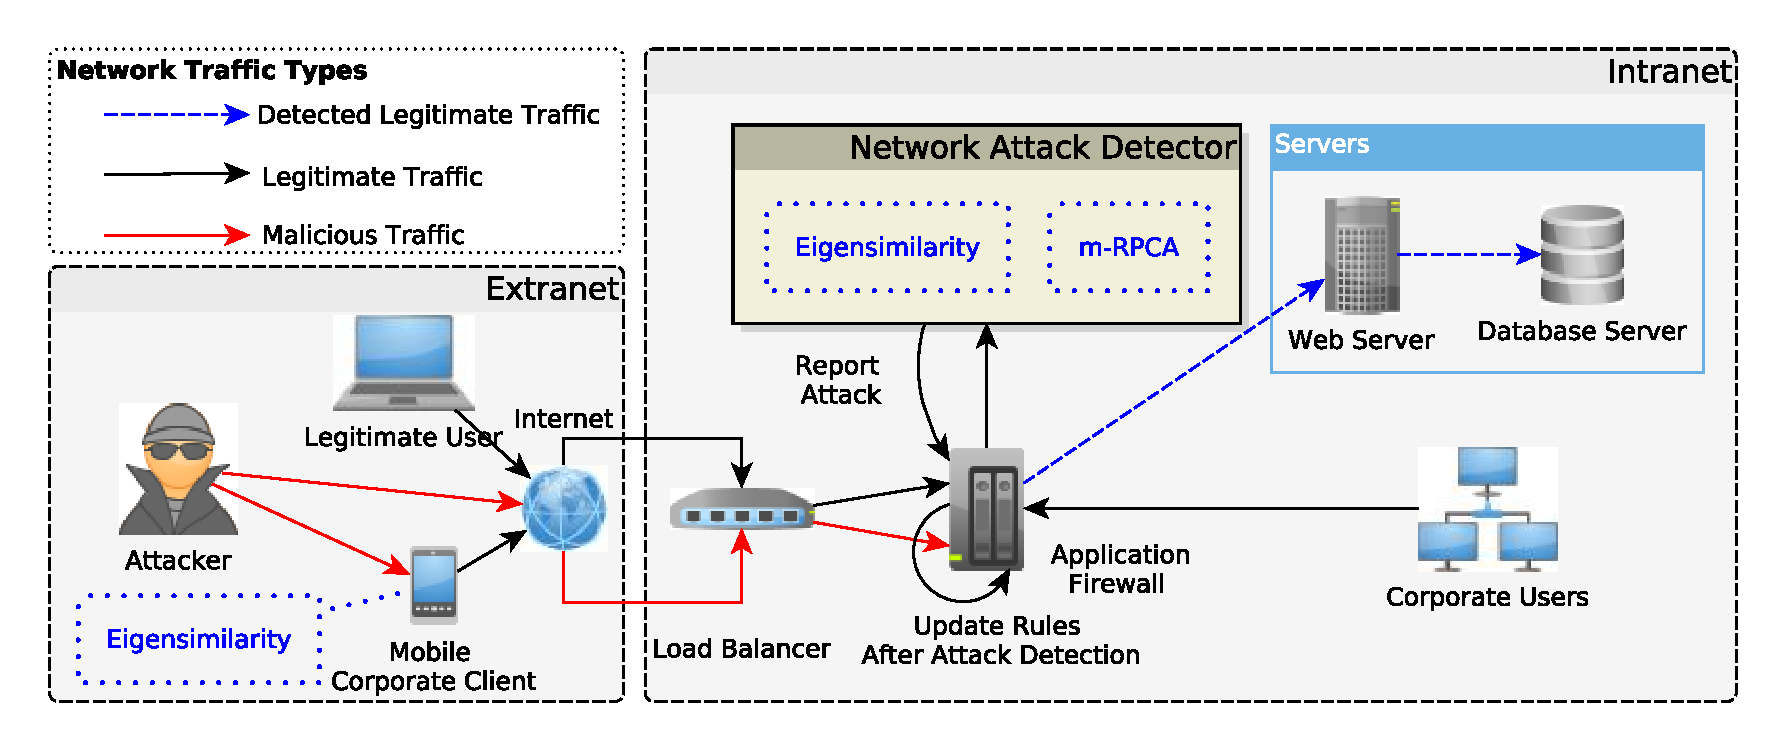
\includegraphics[width=11cm]{figures/ch1/architecture.eps}
    	     \caption{Simplified Architecture for Network Attack Detection.}
    	     \label{fig:2_fig1}
    	\end{figure}
\end{frame}

\begin{frame}[c]{Contributions}
    \begin{itemize}
    	\item T. P. B. Vieira, D. F. Tenório, J. P. C. da Costa, E. P. de Freitas, G. Del Galdo, and R. T.de Sousa Júnior, “\textbf{Model order selection and eigen similarity based framework for detection and identification of network attacks}\textbf{}”, \textit{Journal of Network and ComputerApplications}, vol. 90, pp. 26–41, 2017 \cite{vieira2017model}.
    	\item T. Galibus, T. P. B. Vieira, E. P. de Freitas, R. d. O. Albuquerque, R. T.de Sousa Júnior, V. Krasnoproshin, A. Zaleski, H. Vissia, G. del Galdoet al., “\textbf{Offline mode for corporate mobile client security architecture}”, \textit{Mobile Networks and Applications}, pp. 1–17, 2017 \cite{galibus2017offline}.
    \end{itemize}
\end{frame}

\begin{frame}[c]{Contributions - Appendix}
    \begin{itemize}
    	\item K. H. C. Ramos, T. P. B. Vieira, J. P. C. L. da Costa, and R. T. de Sousa Júnior, “\textbf{Multidimensional analysis of critical success factors for it governance within the Brazilian federal public administration in the Light of External Auditing Data}". \textit{12th International CONTECSI}, 2015
    	\cite{ramos2015}.
    	\item T. P. B. Vieira, J. P. C. L. da Costa, E. S. C. Vilaça, E. S. Gualberto, and R. T.de Sousa Júnior, “\textbf{Moment distances from robust subspace for network attack detection}”, \textit{Journal of Network and Computer Applications}, \textbf{To Appear} \cite{vieira2019moment}.
    \end{itemize}
\end{frame}

%Eigensimilarity-=-=-=-=-=-=-=-=-=-=-=-=-=-=-=-=-=-=-=-=-=-=-=-=-=-=-=-=-=-=-=-=-=-=-=-=-=-=-=-=-=-=-=-=-=-=-
\section{Eigensimilarity based Framework for Detection and Identification of Network Attacks}

\begin{frame}[c]{Introduction}
	\begin{itemize}
		\item \textbf{DDoS} attacks are continuing to \textbf{rise};
		\item \textbf{Solutions} for monitoring and mitigation of \textbf{DDoS} in \textbf{application layer} start with \textbf{behavioral analytics} and supplement with \textbf{signature-based} detection \cite{Hevesi2019}.
	\end{itemize}
\end{frame}

\begin{frame}[c]{Introduction}
	\begin{itemize}
        \item \textbf{Probe} attacks aim to \textbf{scan} networks to identify \textbf{opportunities};
        \item A \textbf{probe attack} is considered the \textbf{first step} in an attack;
        \item \textbf{Probe} attacks are considered \textbf{serious threats} by \cite{ahmed2016survey} and \cite{moustafa2019holistic}.
	\end{itemize}
\end{frame}

\begin{frame}[c]{Introduction}
    We propose the Eigensimilarity:
	\begin{itemize}
		\item \textbf{MOS} and \textbf{eigenvalue analysis} are applied to detect \textbf{time frames under attack};
		\item \textbf{Eigenvector similarity analysis} is used for extracting detailed time and network ports under attack;
		\item We evaluate the \textbf{computational complexity} and the required \textbf{processing time}.
	\end{itemize}
\end{frame}

\begin{frame}[c]{Related works}
	\begin{itemize}
		\item Callegari \emph{et al} \cite{Zonglin2009} propose a \textbf{PCA-based} method for identifying the traffic flows responsible for an anomaly detected at the aggregate level. However, Callegari \emph{et al} \textbf{focus on flood attack detection, not addressing probe} attack detection, and their approach \textbf{relies on visual analysis}.
		\item Lu and Ghorbani \cite{Lu2009} proposed a \textbf{network anomaly} detection model based on \textbf{network flow, wavelet approximation, and system identification theory}. However, their work requires a \textbf{training} and presents \textbf{limitations} on identification of behaviors without \textbf{significant outliers}.
	\end{itemize}
\end{frame}

% \begin{frame}[c]{Related works}
% 	\begin{itemize}
% 		\item Lee \emph{et al.} \cite{Lee2013} propose OverSampling PCA, determines the \textbf{anomaly} according to the variation of \textbf{eigenvector by similarity analysis and over sampling}. We apply \textbf{MOS for attack detection} and \textbf{similarity analysis for identification} of time and ports under attack;
% 	\end{itemize}
% \end{frame}

\begin{frame}{data sets}
	We focus on \textbf{probe} and \textbf{flooding} attacks for two scenarios: 
	\begin{itemize}
		\item A \textbf{synthetic data set} as a signal superposition of legitimate traffic and malicious traffic;
		\item Selected cases of \textbf{DARPA data set} that reproduce probe and flooding attacks.
	\end{itemize}
\end{frame}

\begin{frame}{Data Model}
	Network traffic as a signal superposition matrix:
	\begin{equation}\label{eq:eq01}
		\boldsymbol{X}^{(q)} = \boldsymbol{U}^{(q)} + \boldsymbol{N}^{(q)},
	\end{equation}
	\begin{itemize}
	    \item $\boldsymbol{X}^{(q)} \in \mathbb{R}^{M \times N}$ has \emph{M} rows and \emph{N} columns;
		\item The data is divided into \textbf{$Q$ time frames};
		\item Each \textbf{row} is a \textbf{TCP/UDP port}, and each \textbf{column} represents \textbf{time} bins (minute);
		\item Each element $x_{m,n}^{(q)}$ stands for the \textbf{number of packets for port $m$ at the $n$-th minute}, at the $q$-th time frame.
	\end{itemize}
\end{frame}

\begin{frame}[c]{Synthetic data set}
	\begin{figure}[h!]
	     \centering
	     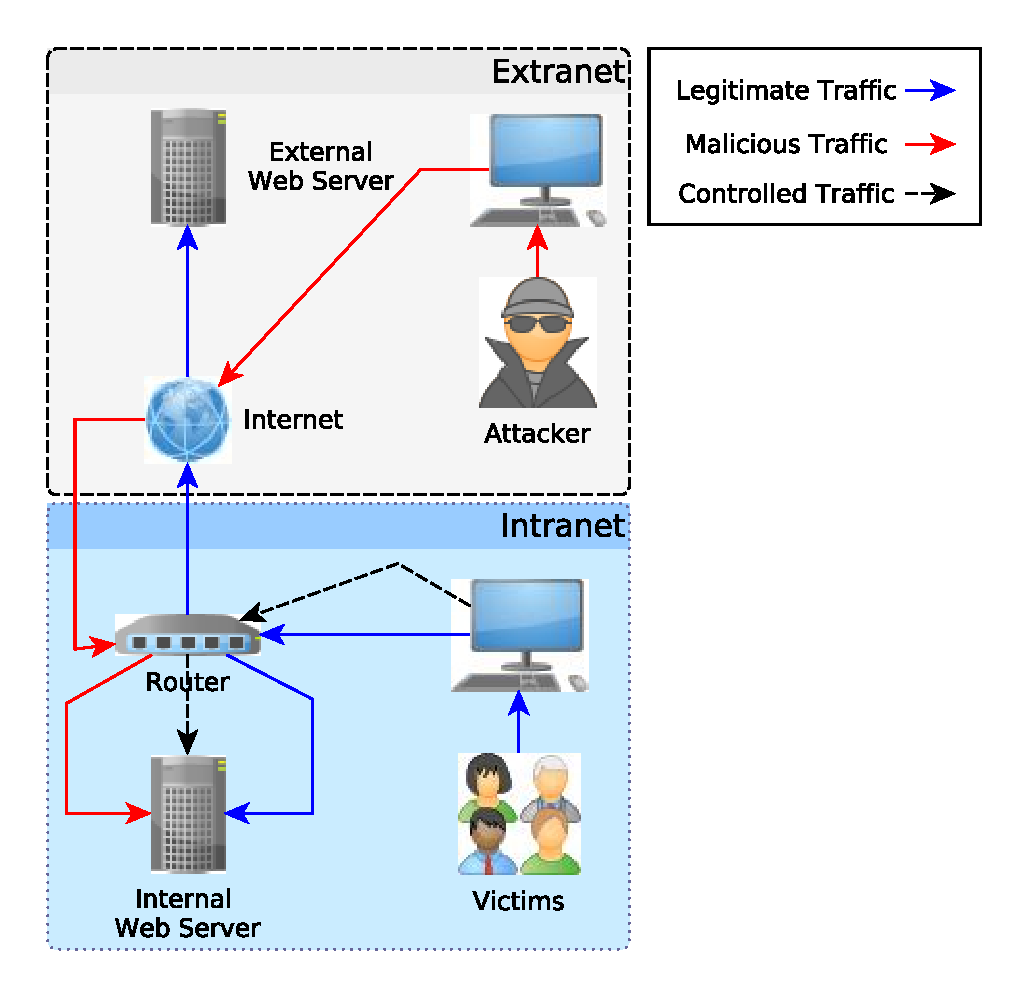
\includegraphics[width=7cm]{figures/ch2/scenario.eps}
	     \caption{Scenario for \textbf{legitimate, synflood, fraggle and port scan attack traffic}.}
	     \label{fig:2_fig1}
	\end{figure}
\end{frame}

\begin{frame}[c]{Synthetic data set}
	\begin{figure}[h!]
	     \centering
	     \includegraphics[width=9cm]{figures/ch2/user_operations.eps}
	     \caption{Scenario with \textbf{legitimate} traffic.}
	     \label{fig:2_fig1}
	\end{figure}
\end{frame}

\begin{frame}[c]{Synthetic data set}
	
	\begin{figure}[h!]
	     \centering 
	     \includegraphics[width=9cm]{figures/ch2/synflood_traffic.eps}
	     \caption{A large quantity of \textbf{SYN} requests, in order to cause a DoS.}
	     \label{fig:2_fig5}
	\end{figure}

\end{frame}

\begin{frame}{DARPA data set}
	\begin{itemize}
	    \item \textbf{7 weeks} of sniffed traffic saved into raw TCPDUMP packet data, from \textbf{inside and outside} origins, with \textbf{labeled} attacks;
	    \item We \textbf{select the cases} that reproduce \textbf{probe and flooding} attacks, apply a \textbf{packet level} analysis.
	\end{itemize}
\end{frame}

\begin{frame}{Eigensimilarity}
	\begin{figure}[h!]
		\centering
	     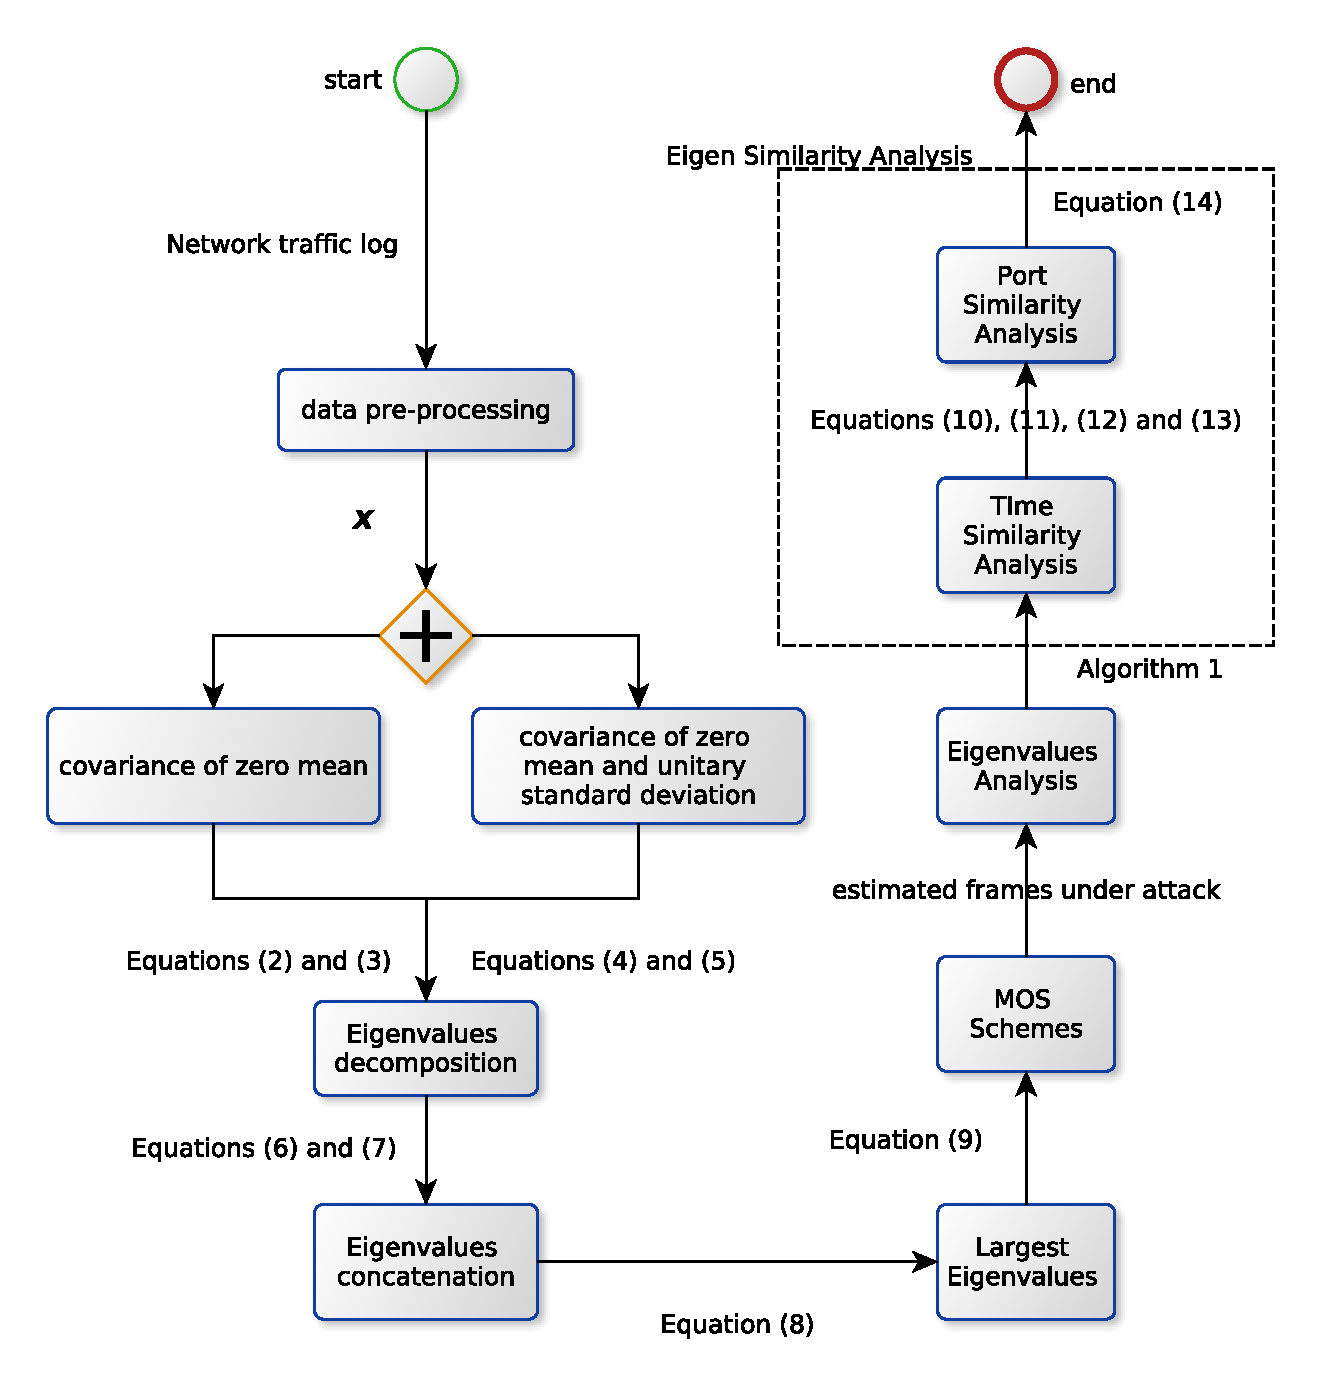
\includegraphics[width=7cm]{figures/ch2/mos_eigen_similarity.eps}
	     \caption{Overview of The Framework for Detection and Identification of Network Attacks.}
	     \label{fig:2_fig80}
	\end{figure}
\end{frame}

% \begin{frame}{Eigensimilarity}
% 	For \textbf{flooding} detection, calculate the \textbf{sample covariance matrix} $\boldsymbol{\hat{R}}_{yy}^{(q)}$ of the \textbf{zero mean samples} given by
% 	\begin{equation}\label{eq:eq02}
% 		\boldsymbol{y}_{m}^{(q)} = \boldsymbol{x}_{m}^{(q)} - \bar{\boldsymbol{x}}_{m}^{(q)}.
% 	\end{equation}
% 	the sample covariance matrix $\boldsymbol{\hat{R}}_{yy}^{(q)}$ can be calculated as follows
% 	\begin{equation}\label{eq:eq03}
% 		\boldsymbol{\hat{R}}_{yy}^{(q)} = \frac{1}{N}\boldsymbol{Y}^{(q)}\boldsymbol{Y}^{(q)^{\rm T}}.
% 	\end{equation}
% \end{frame}

% \begin{frame}{Eigensimilarity}
% 	For \textbf{probing} detection, compute the \textbf{sample covariance} $\boldsymbol{\hat{R}}_{zz}^{(q)}$ whose variables have \textbf{zero mean and unitary standard deviation} as follows
% 	\begin{equation}\label{eq:eq04}
% 		\boldsymbol{z}_{m}^{(q)} = \frac{\boldsymbol{x}_{m}^{(q)} - \bar{\boldsymbol{x}}_{m}^{(q)}}{\boldsymbol{\sigma}_{m}^{(q)}}.
% 	\end{equation}
% 	The sample covariance matrix $\boldsymbol{\hat{R}}_{zz}^{(q)}$ can be calculated via 
% 	\begin{equation}\label{eq:eq05}
% 		\boldsymbol{\hat{R}}_{zz}^{(q)} = \frac{1}{N}\boldsymbol{Z}^{(q)}\boldsymbol{Z}^{(q)^{\rm T}}.
% 	\end{equation}
% \end{frame}

% \begin{frame}{Eigensimilarity}
% 	We refer to $\boldsymbol{\hat{R}}_{yy}$ and $\boldsymbol{\hat{R}}_{zz}$ as a matrix $\boldsymbol{\hat{R}}$
% 	Compute eigenvalue decomposition (EVD) to obtain the vector of eigenvalues $\boldsymbol{e}^{(q)}$ associated with each matrix (time frame $q$), according to (\ref{eq:eq060}).
% 	\begin{equation}\label{eq:eq06}
% 	\boldsymbol{\hat{R}}^{(q)} = \boldsymbol{V}^{(q)}\boldsymbol{\Lambda}^{(q)}\boldsymbol{V}^{(q)^{\rm T}},
% 	\end{equation}
% 	\begin{equation}\label{eq:eq060}
% 	\boldsymbol{e}^{(q)} = \rm diag(\boldsymbol{\Lambda}^{(q)}),
% 	\end{equation}
% 	The eigenvalues should be sorted in descending order, i.e., $\lambda_{1}^{(q)} > \lambda_{2}^{(q)} > \lambda_{3}^{(q)} > ... > \lambda_{m}^{(q)}$.
% \end{frame}

% \begin{frame}{Eigensimilarity}
% 	\begin{equation}\label{eq:eq07}
% 		\boldsymbol{E} =
% 		\begin{bmatrix}
% 			\color{red}\lambda_1^{(1)} & \color{red}\lambda_1^{(2)} & \color{red}\lambda_1^{(3)} & \cdots & \color{red}\lambda_1^{(Q)} \\
% 			\lambda_2^{(1)} & \lambda_2^{(2)} & \lambda_2^{(3)} & \cdots & \lambda_2^{(Q)} \\
% 			\lambda_3^{(1)} & \lambda_3^{(2)} & \lambda_3^{(3)} & \cdots & \lambda_3^{(Q)} \\
% 			\vdots & \vdots & \ddots & \vdots  \\
% 			\lambda_m^{(1)} & \lambda_m^{(2)} & \lambda_m^{(3)} & \cdots & \lambda_m^{(Q)} \\
% 		\end{bmatrix}.
% 	\end{equation}
% 	\begin{equation}\label{eq:eq08}
% 		\boldsymbol{e}_{\rm max} = [ \lambda_1^{(1)}, \lambda_1^{(2)} ... \lambda_1^{(Q)}]
% 	\end{equation}
% \end{frame}

% \begin{frame}{MOS Scheme}
% 	\begin{itemize}
% 		\item $\boldsymbol{e}_{\rm max}$ is sorted in descending order, producing $\sim\boldsymbol{e}_{\rm max}$, that is used as input parameter for MOS schemes;
% 		\item $\hat{d} = \rm{MOS}(\sim\boldsymbol{e}_{\rm max})$.
% 		\item $\hat{d}$ is the estimated \textbf{number of time frames under attack}.
% 	\end{itemize}
% \end{frame}

% \begin{frame}{Eigenvalue Analysis}
% 	\textbf{Eigenvalue analysis} identifies the \textbf{time frames} $q$ under attack.
% 	\begin{figure}[h!]
% 	     \centering 
% 	     \includegraphics[width=8cm]{figures/ch2/alg.png}
% 	     \label{fig:2_fig91}
% 	\end{figure}
% \end{frame}

\begin{frame}{Eigenvector Similarity Analysis}
	\textbf{Eigenvector Similarity} identifies the attacked \textbf{time and ports}.
	\begin{itemize}
	    \item \textbf{Low similarity} between the most significant eigenvectors can highlight anomalies inserted by \textbf{network attacks};
	\end{itemize}
	\begin{equation}
		\label{eq:eq11}
		s_n = \frac{\abs{\boldsymbol{v}^{(q)} \cdot \boldsymbol{v}_{(n)}}}{\norm{\boldsymbol{v}^{(q)}}\norm{\boldsymbol{v}_{(n)}}};
	\end{equation}	
	\begin{itemize}
	    \item $s_n$ denotes the absolute \textbf{similarity} degree of the $n$-th minute;
	    \item $\boldsymbol{v}^{(q)}$ is the \textbf{legitimate} most significant eigenvectors;
	    \item $\boldsymbol{v}_{(n)}$ is the most \textbf{significant eigenvectors} obtained after append the target $n$-th minute for \textbf{testing}.
	\end{itemize}
\end{frame}

\begin{frame}{Eigenvector Similarity Analysis}
	\begin{itemize}
	    \item $\boldsymbol{X}^{(q)}$ is a time frame estimated as \textbf{legitimate};
	    \item Each $\boldsymbol{x}^{(\hat{q})}_{(n)}$ vector of each $n$-th minutes of the estimated $\rm{\boldsymbol{\hat{q}}}_{\rm max}$ time frame shall be individually appended into $\boldsymbol{X}^{(q)}$, as
	\end{itemize}
	\begin{equation}\label{eq:eq12}
		\boldsymbol{X}_{n} = \{\boldsymbol{X}^{(q)} | \boldsymbol{x}^{(\hat{q})}_{(n)}\};
	\end{equation}
	\begin{itemize}
	    \item $\boldsymbol{v}_{(q)}$ is computed from $\boldsymbol{X}_{(q)}$;
	    \item $\boldsymbol{v}_{(n)}$ is computed from $\boldsymbol{X}_{(n)}$;
	    \item $\boldsymbol{s}_{(n)}$ is computed from $\boldsymbol{v}_{(q)}$ and $\boldsymbol{v}_{(n)}$;
	    \item Low $\boldsymbol{s}_{(n)}$ identifies a $n$-th\textbf{ minute under attack}.
	\end{itemize}
\end{frame}

\begin{frame}{Eigenvector Similarity Analysis}
	We propose and evaluate \textbf{three approaches} for eigenvector similarity analysis: 
	\begin{itemize}
		\item \textbf{incremental:} concatenates $\boldsymbol{x}^{(\hat{q})}_{(n)}$ incrementally into $\boldsymbol{X}^{(q)}$;
		\item \textbf{individual:} concatenates each $\boldsymbol{x}^{(\hat{q})}_{(n)}$ individually into $\boldsymbol{X}^{(q)}$;
		\item \textbf{incremental individualized:} concatenates $\boldsymbol{x}^{(\hat{q})}_{(n)}$ incrementally into $\boldsymbol{X}^{(q)}$ until attack detection. Afterwards, concatenates each $\boldsymbol{x}^{(\hat{q})}_{(n)}$ individually into $\boldsymbol{X}^{(q)}$.
	\end{itemize}
\end{frame}

\begin{frame}{Eigenvector Similarity Analysis}
	\begin{figure}[h!]
		\centering
	    \includegraphics[width=11.5cm]{figures/ch2/incremental.eps}
	    \caption{Traffic selection for incremental approach.}
	    \label{fig:2_fig8}
	\end{figure}
\end{frame}

\begin{frame}{Eigenvector Similarity Analysis}
	\begin{figure}[h!]
	     \includegraphics[width=11.5cm]{figures/ch2/individualized.eps}
	     \caption{Traffic selection for individual approach.}
	     \label{fig:2_fig9}
	\end{figure}
\end{frame}

\begin{frame}{Eigenvector Similarity Analysis}
	\begin{figure}[h!]
	     \includegraphics[width=11.5cm]{figures/ch2/incremental_individualized.eps}
	     \caption{Traffic selection for incremental individualized approach.}
	     \label{fig:2_fig2}
	\end{figure}
\end{frame}

\begin{frame}{Eigenvector Similarity Analysis}
	\textbf{Detection of ports under attack}:
	\begin{itemize}
		\item The $\boldsymbol{v}^{(q)}$ last most significant eigenvectors without attack is compared against the $\boldsymbol{v}_{(n)}$ identified as under attack;
		\item Evaluate the cosine similarity of each $m$-th port of all $\boldsymbol{\hat{n}}$ minutes identified as under attack.
	\end{itemize}
	\begin{equation}\label{eq:eq15}
		\left\{
		\begin{array}{@{}ll@{}}
			x_{(m,n)} = x^{(\hat{q})}_{(m,\hat{n})} \\
			\\
			s_{m,\hat{n}} = \frac{\abs{\boldsymbol{v}^{(q)} \cdot \boldsymbol{v}_{(m,\hat{n})}}}{\norm{\boldsymbol{v}^{(q)}}\norm{\boldsymbol{v}_{(m,\hat{n})}}},
		\end{array}\right.
	\end{equation}
	\begin{itemize}
		\item Low $\boldsymbol{s}_{m,\hat{n}}$ identifies a $m$-th \textbf{port under attack} during the $n$-th minute.
	\end{itemize}
\end{frame}

\begin{frame}{Results - synthetic data set}
	\begin{table}[h!]
	  \centering
	  \scriptsize
	  \caption{Largest Eigenvalue related to attacks detection}
	  \label{tab:tab3}
	  \begin{tabular}{ c c c c c }
		\toprule
		\multirow{3}{*}{\textbf{Time Frame} $q$} &\multicolumn{4}{c }{\textbf{Vectors GETV}}\\ 
				\hhline{~----}
			&\textbf{Detection of}	 &\textbf{Detection of}	 &\textbf{Detection of}	 &\textbf{Detection of}\\
			&\textbf{\emph{synflood/fraggle}}	 &\textbf{\emph{synflood}}	 &\textbf{\emph{fraggle}}	 &\textbf{\emph{port scan}}\\
		\midrule
		1 &1887545 &1887545 &1887545 &2,0734 \\
		2 &2341327 &2341327 &2341327 &2,1451 \\
		3 &3213867 &3213867 &3213867 &\color{red}10,0718 \\
		4 &\color{red}133238294 &\color{red}133238294 &731229 &2,1620 \\
		5 &\color{red}92384021611 &6367983 &\color{red}92384021611 &2,4253 \\
		6 &708335 &708335 &708335 &1,7948 \\
	    \bottomrule
	  \end{tabular}
	\end{table}
\end{frame}

\begin{frame}{Results - synthetic data set}
	\begin{table}[h!]
	  \centering
	  \tiny
	  \caption{MOS schemes applied to port scan and flood detection}
	  \label{tab:tab4}
	  \begin{tabular}{ c c c c c c c c }
		\toprule
		\multirow{2}{*}{\textbf{Type of analysis} $q$} &\multicolumn{6}{c}{\textbf{MOS schemes (estimated model order $\hat{d}$)}} &{\textbf{(d)}}\\ 
				\hhline{~------~}
			&\textbf{AIC} &\textbf{MDL} &\textbf{EDC} &\textbf{RADOI} &\textbf{EFT} &\textbf{SURE}\\
		\midrule
		Detection of synflood \\(presence of attack) &2 &1 &\textbf{\color{red}1} &5 &\textbf{\color{red}1} &4 &\textbf{\color{red}1} \\
		Detection of synflood \\(absence of attack) &1 &1 &\textbf{\color{red}0} &1 &\textbf{\color{red}0} &3 &\textbf{\color{red}0} \\
		\midrule
		Detection of fraggle \\(presence of attack) &1 &1 &\textbf{\color{red}1} &5 &\textbf{\color{red}1} &4 &\textbf{\color{red}1} \\
		Detection of fraggle \\(absence of attack) &1 &1 &\textbf{\color{red}0} &1 &\textbf{\color{red}0} &3 &\textbf{\color{red}0} \\
		\midrule
		Detection of port scan \\(presence of attack) &1 &1 &\textbf{\color{red}1} &1 &\textbf{\color{red}1} &9 &\textbf{\color{red}1} \\
		Detection of port scan \\(absence of attack) &0 &0 &\textbf{\color{red}0} &1 &\textbf{\color{red}0} &1 &\textbf{\color{red}0} \\
		\midrule
		Detection of synflood/fraggle \\(presence of attack) &2 &2 &\textbf{\color{red}2} &5 &\textbf{\color{red}2} &5 &\textbf{\color{red}2} \\
		Detection of synflood/fraggle \\(absence of attack) &1 &1 &\textbf{\color{red}0} &1 &\textbf{\color{red}0} &3 &\textbf{\color{red}0} \\
	    \bottomrule
	  \end{tabular}
	\end{table}
\end{frame}

\begin{frame}{Results - synthetic data set}
	\begin{table}[h!]
	  \centering
	  \tiny
	  \caption{Eigenvector Similarity Analysis for Port Scan Detection}
	  \label{tab:tab5}
	  \begin{tabular}{ c c c c c c }
		\toprule
		\multirow{2}{*}{\textbf{Time Frame} $q$} &\multirow{2}{*}{\textbf{Time} $n$}   &\multicolumn{3}{c}{\textbf{Similarity Analysis}} &\multirow{2}{*}{\textbf{Attack?}}\\ 
				\hhline{~~---~}
				& &\textbf{Incremental Individualized} &\textbf{Incremental} &\textbf{Individual}\\
		\midrule
		3 &1 &0.9946 &0.9946 &0.9946 &no \\
		3 &2 &0.9934 &0.9934 &0.9999 &no \\
		3 &3 &0.9912 &0.9912 &0.9999 &no \\
		3 &4 &0.9888 &0.9888 &0.9999 &no \\
		3 &5 &0.9856 &0.9856 &0.9998 &no \\
		3 &6 &0.9840 &0.9840 &0.9999 &no \\
		3 &7 &0.9824 &0.9824 &1.0000 &no \\
		3 &8 &0.9794 &0.9794 &0.9999 &no \\
		3 &9 &0.9673 &0.9673 &0.9926 &no \\
		3 &10 &0.9674 &0.9674 &0.9997 &no \\
		3 &11 &0.9733 &0.9733 &0.9993 &no \\
		3 &12 &0.9702 &0.9702 &0.9993 &no \\
		3 &13 &0.9677 &0.9677 &0.9999 &no \\
		3 &14 &0.9646 &0.9646 &0.9998 &no \\
		3 &15 &\color{red}0.0216 &\color{red}0.0216 &\color{red}0.0276 &\color{red}yes \\
		3 &16 &0.9621 &\color{red}0.0209 &1.0000 &no \\
		3 &17 &0.9611 &\color{red}0.0199 &0.9998 &no \\
		3 &18 &0.9612 &\color{red}0.0191 &0.9999 &no \\
		3 &19 &0.9613 &\color{red}0.0186 &0.9998 &no \\
		3 &20 &0.9638 &\color{red}0.0190 &1.0000 &no \\
	    \bottomrule
	  \end{tabular}
	\end{table}	
\end{frame}

%\begin{frame}{Results - synthetic data set}
%	\begin{table}[h!]
%	  \centering
%	  \tiny
%	  \caption{Eigenvector Similarity Analysis for Synflood Detection}
%	  \label{tab:tab6}
%	  \begin{tabular}{ c c c c c c }
%		\toprule
%		\multirow{2}{*}{\textbf{Time Frame} $q$} &\multirow{2}{*}{\textbf{Time} $n$}   &\multicolumn{3}{c}{\textbf{Similarity Analysis}} &\multirow{2}{*}{\textbf{Attack?}}\\ 
%				\hhline{~~---~}
%				& &\textbf{Incremental Individualized} &\textbf{Incremental} &\textbf{Individual}\\
%		\midrule
%		4 &1 &1.0000 &1.0000 &1.0000 &no \\
%		4 &2 &0.9999 &0.9999 &1.0000 &no \\
%		4 &3 &0.9997 &0.9997 &0.9999 &no \\
%		4 &4 &0.9998 &0.9998 &1.0000 &no \\
%		4 &5 &0.9965 &0.9965 &0.9908 &no \\
%		4 &6 &0.9975 &0.9975 &1.0000 &no \\
%		4 &7 &0.9977 &0.9977 &1.0000 &no \\
%		4 &8 &0.9980 &0.9980 &1.0000 &no \\
%		4 &9 &0.9987 &0.9987 &0.9999 &no \\
%		4 &10 &0.9991 &0.9991 &1.0000 &no \\
%		4 &11 &\color{red}0.0085 &\color{red}0.0085 &\color{red}0.0284 &\color{red}yes \\
%		4 &12 &\color{red}0.0162 &\color{red}0.0120 &\color{red}0.0343 &\color{red}yes \\
%		4 &13 &\color{red}0.0248 &\color{red}0.0158 &\color{red}0.0427 &\color{red}yes \\
%		4 &14 &\color{red}0.1243 &\color{red}0.0185 &\color{red}0.1041 &\color{red}yes \\
%		4 &15 &\color{red}0.0082 &\color{red}0.0162 &\color{red}0.0103 &\color{red}yes \\
%		4 &16 &\color{red}0.0404 &\color{red}0.0070 &\color{red}0.0580 &\color{red}yes \\
%		4 &17 &\color{red}0.0397 &\color{red}0.0007 &\color{red}0.0573 &\color{red}yes \\
%		4 &18 &\color{red}0.0408 &\color{red}0.0042 &\color{red}0.0584 &\color{red}yes \\
%		4 &19 &\color{red}0.0408 &\color{red}0.0079 &\color{red}0.0584 &\color{red}yes \\
%		4 &20 &\color{red}0.0477 &\color{red}0.0092 &\color{red}0.0757 &\color{red}yes \\
%	    \bottomrule
%	  \end{tabular}
%	\end{table}	
%\end{frame}

%\begin{frame}{Results - synthetic data set}
%	\begin{table}[h!]
%	  \centering
%	  \tiny
%	  \caption{Eigenvector Similarity Analysis for Fraggle Detection}
%	  \label{tab:tab7}
%	  \begin{tabular}{ c c c c c c }
%		\toprule
%		\multirow{2}{*}{\textbf{Time Frame} $q$} &\multirow{2}{*}{\textbf{Time} $n$}   &\multicolumn{3}{c}{\textbf{Similarity Analysis}} &\multirow{2}{*}{\textbf{Attack?}}\\ 
%				\hhline{~~---~}
%				& &\textbf{Incremental Individualized} &\textbf{Incremental} &\textbf{Individual}\\
%		\midrule
%		5 &1 &1.0000 &1.0000 &1.0000 &no \\
%		5 &2 &0.9999 &0.9999 &1.0000 &no \\
%		5 &3 &1.0000 &1.0000 &1.0000 &no \\
%		5 &4 &0.9999 &0.9999 &1.0000 &no \\
%		5 &5 &0.9993 &0.9993 &0.9997 &no \\
%		5 &6 &0.9993 &0.9993 &0.9997 &no \\
%		5 &7 &0.9994 &0.9994 &1.0000 &no \\
%		5 &8 &0.9995 &0.9995 &1.0000 &no \\
%		5 &9 &0.9995 &0.9995 &1.0000 &no \\
%		5 &10 &0.9995 &0.9995 &1.0000 &no \\
%		5 &11 &\color{red}0.0031 &\color{red}0.0031 &\color{red}0.0021 &\color{red}yes \\
%		5 &12 &\color{red}0.0019 &\color{red}0.0025 &\color{red}0.0009 &\color{red}yes \\
%		5 &13 &\color{red}0.0030 &\color{red}0.0026 &\color{red}0.0020 &\color{red}yes \\
%		5 &14 &\color{red}0.0030 &\color{red}0.0027 &\color{red}0.0020 &\color{red}yes \\
%		5 &15 &\color{red}0.0030 &\color{red}0.0028 &\color{red}0.0020 &\color{red}yes \\
%		5 &16 &\color{red}0.0012 &\color{red}0.0025 &\color{red}0.0002 &\color{red}yes \\
%		5 &17 &\color{red}0.0030 &\color{red}0.0026 &\color{red}0.0020 &\color{red}yes \\
%		5 &18 &\color{red}0.0030 &\color{red}0.0026 &\color{red}0.0020 &\color{red}yes \\
%		5 &19 &\color{red}0.0030 &\color{red}0.0027 &\color{red}0.0020 &\color{red}yes \\
%		5 &20 &\color{red}0.0069 &\color{red}0.0023 &\color{red}0.0083 &\color{red}yes \\
%	    \bottomrule
%	  \end{tabular}
%	\end{table}
%\end{frame}

%\begin{frame}{Results - synthetic data set}
%	\begin{table}[h!]
%	  \centering
%	  \tiny
%	  \caption{Eigenvector Similarity Analysis for Detection of Ports Under Port Scan Attack (q=3 and n%=15)}
%	  \label{tab:tab8}
%	  \begin{tabular}{ c c c c }
%		\toprule
%		\multirow{2}{*}{\textbf{Port} $p$}   &\multicolumn{2}{c}{\textbf{Approaches}} &\multirow{2}{*}{\textbf{Attack?}}\\ 
%				\hhline{~--~}
%				&\textbf{Incremental Individualized} &\textbf{Individual}\\
%		\midrule
%		80 &0.9999 &0.9999 &no \\
%		443 &0.9999 &0.9999 &no \\
%		53 &0.9999 &0.9999 &no \\
%		21 &0.9999 &0.9997 &\color{red}yes \\
%		22 &\color{red}0.0298 &0.9997 &\color{red}yes \\
%		23 &\color{red}0.0298 &0.9997 &\color{red}yes \\
%		25 &\color{red}0.0298 &0.9997 &\color{red}yes \\
%		110 &\color{red}0.0298 &0.9997 &\color{red}yes \\
%		143 &\color{red}0.0298 &0.9997 &\color{red}yes \\
%		161 &\color{red}0.0298 &0.9997 &\color{red}yes \\
%		69 &\color{red}0.0298 &0.9997 &\color{red}yes \\
%		123 &\color{red}0.0298 &0.9997 &\color{red}yes \\
%		445 &\color{red}0.0298 &0.9997 &\color{red}yes \\
%		600 &0.9999 &0.9999 &no \\
%		19 &0.9999 &0.9999 &no \\
%		67 &0.9999 &0.9999 &no \\
%		68 &0.9999 &0.9999 &no \\
%	    \bottomrule
%	  \end{tabular}
%	\end{table}
%\end{frame}

%\begin{frame}{Results - synthetic data set}
%	\begin{table}[h!]
%	  \centering
%	  \tiny
%	  \caption{Eigenvector Similarity Analysis for Detection of Ports Under Synflood Attack (q=4 and n=11)}
%	  \label{tab:tab9}
%	  \begin{tabular}{ c c c c }
%		\toprule
%		\multirow{2}{*}{\textbf{Port} $p$}   &\multicolumn{2}{c}{\textbf{Approaches}} &\multirow{2}{*}{\textbf{Attack?}}\\ 
%				\hhline{~--~}
%				&\textbf{Incremental Individualized} &\textbf{Individual}\\
%		\midrule
%		80 &1.0000 &1.0000 &no \\
%		443 &1.0000 &1.0000 &no \\
%		53 &1.0000 &1.0000 &no \\
%		21 &1.0000 &1.0000 &no \\
%		22 &1.0000 &1.0000 &no \\
%		23 &1.0000 &1.0000 &no \\
%		25 &1.0000 &1.0000 &no \\
%		110 &1.0000 &1.0000 &no \\
%		143 &1.0000 &1.0000 &no \\
%		161 &1.0000 &1.0000 &no \\
%		69 &1.0000 &1.0000 &no \\
%		123 &1.0000 &1.0000 &no \\
%		445 &1.0000 &1.0000 &no \\
%		600 &\color{red}0.0077 &\color{red}0.0427 &\color{red}yes \\
%		19 &1.0000 &1.0000 &no \\
%		67 &1.0000 &1.0000 &no \\
%		68 &1.0000 &1.0000 &no \\
%	    \bottomrule
%	  \end{tabular}
%	\end{table}
%\end{frame}

%\begin{frame}{Results - synthetic data set}
%	\begin{table}[h!]
%	  \centering
%	  \tiny
%	  \caption{Eigenvector Similarity Analysis for Detection of Ports Under Fraggle Attack (q=5 and t=11)}
%	  \label{tab:tab10}
%	  \begin{tabular}{ c c c c }
%		\toprule
%		\multirow{2}{*}{\textbf{Port} $p$}   &\multicolumn{2}{c}{\textbf{Approaches}} &\multirow{2}{*}{\textbf{Attack?}}\\ 
%				\hhline{~--~}
%				&\textbf{Incremental Individualized} &\textbf{Individual}\\
%		\midrule
%		80 &1.0000 &1.0000 &no \\
%		443 &1.0000 &1.0000 &no \\
%		53 &1.0000 &1.0000 &no \\
%		21 &1.0000 &1.0000 &no \\
%		22 &1.0000 &1.0000 &no \\
%		23 &1.0000 &1.0000 &no \\
%		25 &1.0000 &1.0000 &no \\
%		110 &1.0000 &1.0000 &no \\
%		143 &1.0000 &1.0000 &no \\
%		161 &1.0000 &1.0000 &no \\
%		69 &1.0000 &1.0000 &no \\
%		123 &1.0000 &1.0000 &no \\
%		445 &1.0000 &1.0000 &no \\
%		600 &1.0000 &1.0000 &no \\
%		19 &\color{red}0.0031 &\color{red}0.0004 &\color{red}yes \\
%		67 &1.0000 &1.0000 &no \\
%		68 &1.0000 &1.0000 &no \\
%	    \bottomrule
%	  \end{tabular}
%	\end{table}
%\end{frame}

\begin{frame}{Results - synthetic data set}
	For \textbf{time} attack detection:
	\begin{itemize}
		\item \textbf{High similarity} between network traffic \textbf{without attack} (0.9610) and \textbf{low similarity} with \textbf{attack} (0.0276);
		\item The \textbf{incremental} approach produces \textbf{false positive} results.
	\end{itemize}
	For \textbf{port} attack detection:
	\begin{itemize}
		\item The \textbf{incremental individualized} has more \textbf{sensibility} to anomaly detection;
		\item The \textbf{individual} approach \textbf{was not able} to identify low similarity for ports under attack;
	\end{itemize}
\end{frame}

\begin{frame}{Results - synthetic data set}
    Hypothesis evaluation:
	\begin{itemize}
		\item The results answer positively the question $Q_1$ ("\textbf{Can the analysis of patterns from a learned subspace identify and detect anomalies in network traffic?}");
		\item The results rejects the null hypothesis $H_1^{(N)}$ and confirms the alternative hypothesis $H_1^{(A)}$ ("\textbf{A subspace learned by eigenvalue decomposition can be used to detect and identify network attacks}").
	\end{itemize}
\end{frame}

\begin{frame}{Results - DARPA data set}
	\begin{table}[!t]
		\caption{Results of the attack detection evaluation}
		\label{tab:tab12}
		\centering
		\scriptsize
		\begin{tabular}{|c|c|c|c|c|}
			\hline \rowcolor{Gray} \begin{tabular}[x]{@{}l@{}}Solution\end{tabular}	& \begin{tabular}[x]{@{}l@{}}Attack Type\end{tabular}	 & \begin{tabular}[x]{@{}l@{}}Metric\end{tabular}	& \begin{tabular}[x]{@{}l@{}}Result\end{tabular} \\ \hline
			Proposed Work	&Flooding	&True Positive	&100.00 \%\\ \hline
			Proposed Work	&Flooding	&False Positive	&60.00 \%\\ \hline
			Proposed Work	&Flooding	&Misclassification	&50.00 \%\\ \hline
			Proposed Work	&Probe	&True Positive	&76.92 \%\\ \hline
			Proposed Work	&Probe	&False Positive	&18.52 \%\\ \hline
			Proposed Work	&Probe	&Misclassification	&32.73 \%\\ \hline
			Callegari \emph{et al}	&Flooding	&True Positive	&82.00 \%\\ \hline
			Callegari \emph{et al}	&Flooding	&False Positive	&-\\ \hline
			Callegari \emph{et al}	&Flooding	&Misclassification	&-\\ \hline
			Lu and Ghorbani	&Overall	&True Positive	&94.67 \%\\ \hline
			Lu and Ghorbani	&Overall	&False Positive	&-\\ \hline
			Lu and Ghorbani	&Overall	&Misclassification	&-\\ \hline
			Lu and Ghorbani	&Portsweep	&True Positive	&50.00 \%\\ \hline
			Lu and Ghorbani	&Portsweep	&False Positive	&-\\ \hline
			Lu and Ghorbani	&Portsweep	&Misclassification	&-\\ \hline
		\end{tabular}
	\end{table}
\end{frame}

\begin{frame}{Results - DARPA data set}
	% Misclassification is defined as $\frac{(FN+FP)}{(TP+FP+FN+TN)}$;
	\begin{itemize}
		\item \textbf{High FP and misclassification} due to \textbf{massive legitimate traffic} (such as an attack) sometimes;
		\item Callegari \emph{et al} is based on PCA, without training
		\begin{itemize}
			\item \textbf{82 \% while we obtain 100 \%};
			\item \textbf{FP and misclassification was not evaluated}.
		\end{itemize}
		\item Lu and Ghorbani's is based on signal processing and uses DARPA
		\begin{itemize}
			\item 94.67 \% and 50.00 \%, while we obtain \textbf{100 \% and 76.92 \%};
			\item \textbf{FP and misclassification was not evaluated}.
		\end{itemize}
	\end{itemize}
\end{frame}

\begin{frame}{Performance Evaluation}
	Complexity Analysis:
	\begin{itemize}
		\item The worst-case running time is $O(N^3)$;
		\item The computational complexity of \textbf{EVD is predominant};
		\item \textbf{However}, the approach \textbf{splits the data into time frames} with period time $N$, which makes possible to \textbf{limit the growth of $N$}.
	\end{itemize}
\end{frame}

%\begin{frame}{Performance Evaluation}
%	\begin{table}[!t]
%		\caption{Processing time of the main steps for anomaly detection}
%		\label{tab:11}
%		\centering
%		\tiny
%		\begin{tabular}{|r|r|r|r|r|r|r|}
%			\hline \rowcolor{Gray} \begin{tabular}[x]{@{}l@{}}Traffic Time\\(hour)\end{tabular}	& \begin{tabular}[x]{@{}l@{}}Frame Size\\(min)\end{tabular}	 & \begin{tabular}[x]{@{}l@{}}Num. Ports\end{tabular}	& \begin{tabular}[x]{@{}l@{}}1-time\\(ms)\end{tabular}	& \begin{tabular}[x]{@{}l@{}}2-time\\(ms)\end{tabular}	& \begin{tabular}[x]{@{}l@{}}3-time\\(ms)\end{tabular}	\\ \hline
%			16	& 10	& 17	& 0.7900	& 0.8100	& 0.0650\\ \hline
%			16	& 20	& 17	& 0.5250	& 0.5950	& 0.0100\\ \hline
%			16	& 60	& 17	& 0.9700	& 1.1400	& 0.0250\\ \hline
%			16	& 120	& 17	& 0.6050	& 0.6100	& 0.0050\\ \hline
%			16	& 60	& 34	& 1.2750	& 1.2200	& 0.0050\\ \hline
%			16	& 120	& 34	& 1.1200	& 1.1700	& 0.0050\\ \hline
%			20	& 10	& 17	& 2.7950	& 2.8950	& 1.1000\\ \hline
%			20	& 20	& 17	& 2.0700	& 2.0200	& 0.3500\\ \hline
%			20	& 60	& 17	& 1.0250	& 1.0450	& 0.0650\\ \hline
%			20	& 120	& 17	& 1.0000	& 1.0700	& 0.0350\\ \hline
%			20	& 60	& 34	& 2.9650	& 3.2100	& 0.0400\\ \hline
%			20	& 120	& 34	& 2.9950	& 3.1150	& 0.0200\\ \hline
%			22	& 10	& 17	& 4.7250	& 4.0850	& 1.4600\\ \hline
%			22	& 20	& 17	& 2.3200	& 2.6800	& 0.2450\\ \hline
%			22	& 60	& 17	& 1.0700	& 1.1200	& 0.0300\\ \hline
%			22	& 120	& 17	& 0.9900	& 1.0500	& 0.0250\\ \hline
%			22	& 60	& 34	& 3.0850	& 3.1250	& 0.0650\\ \hline
%			22	& 120	& 34	& 2.8100	& 2.9600	& 0.0250\\ \hline
%		\end{tabular}
%	\end{table}
%\end{frame}

\begin{frame}{Performance Evaluation}
	Processing Time Analysis:
	\begin{itemize}
		\item The processing time \textbf{increases according to traffic time}, but the \textbf{worst} processing time is \textbf{4.7250 milliseconds};
		% \item The processing time \textbf{increases} with the frame size $N$ \textbf{decreasing};
		\item The \textbf{number of ports} $M$ increases the \textbf{processing time}.
	\end{itemize}
\end{frame}


%m-RPCA-=-=-=-=-=-=-=-=-=-=-=-=-=-=-=-=-=-=-=-=-=-=-=-=-=-=-=-=-=-=-=-=-=-=-=-=-=-=-=-=-=-=-=-=-=-=-=-=-=-=-=-
\section{Robust Framework for Detection of Network Attacks in Imbalanced Traffic}

\begin{frame}{Introduction}
	\begin{itemize}
		\item \textbf{37.9\%} of all Internet traffic is from \textbf{bots};
		\item \textbf{Anomalies} in network traffic can be \textbf{hard} to identify from legitimate data, due to the \textbf{rare} occurrences;
		\item \textbf{Network anomaly detection} is usually applied to \textbf{imbalanced} data \cite{Phua2004minority};
	\end{itemize}
\end{frame}

\begin{frame}{Introduction}
	\begin{itemize}
		\item \textbf{Imbalanced} data can \textbf{compromise} the performance of most standard \textbf{learning algorithms};
		\item \textbf{Network traffic} is usually characterized by \textbf{skewed and heavy-tailed} distributions \cite{leon2017probability};
		\item Traditionally adopted \textbf{algorithms for anomaly detection} assume a \textbf{Gaussian} or symmetric distributed data \cite{lakhina2005mining}.
	\end{itemize}
\end{frame}

\begin{frame}{Introduction}
    \textbf{Moment-based Robust Principal Component Analysis (m-RPCA)}:
	\begin{itemize}
		\item A \textbf{robust subspace} is computed from \textbf{legitimate observations}, for estimating \textbf{robust moments};
		\item The \textbf{Mahalanobis distance} between the \textbf{robust moments} and \textbf{new contaminated observations} can estimate \textbf{anomalies} in a \textbf{semi-supervised and unsupervised} fashion;
		\item We \textbf{evaluate} m-RPCA for anomaly detection on \textbf{simulated data sets} and for network attack detection on \textbf{CTU-13 data set} \cite{garcia2014empirical};
		\item We \textbf{compare} our proposal to \textbf{widely adopted algorithms} for anomaly detection and to \textbf{ROBPCA}.
	\end{itemize}
\end{frame}

\begin{frame}[c]{Related works}
	\begin{itemize}
	    \item Hubert \emph{et al.} \cite{hubert2009robustskewed} proposed \textbf{ROBPCA-AO}, which improves ROBPCA for problems with skewed data, by means of an adjusted outlyingness based on robust skewness;
		\item Pascoal \emph{et al.} \cite{pascoal2012robust} proposed an approach based on a robust mutual information estimator for feature selection and based on \textbf{RPCA for outlier detection in internet traffic};
		\item Zhou and Paffenroth \cite{zhou2017anomaly} proposed the \textbf{Robust Deep Autoencoders (RDA)}, which inherits the \textbf{non-linear representation} capabilities of \textbf{autoencoders} combined with the \textbf{outlier separation of RPCA}. 
	\end{itemize}
\end{frame}

\begin{frame}[c]{Data Set - Simulated}
    \textbf{We propose to evaluate m-RPCA for anomaly detection on simulated data}:
	\begin{itemize}
		\item Two data sets with \textbf{skewed and heavy tailed distributions}:
		\begin{itemize}
    		\item Pareto and Gaussian anomalies;
    		\item Lognormal and Gaussian anomalies;
		\end{itemize}
		\item Gaussian distributed data set, to evaluate m-RPCA for general purposes:
    		\begin{itemize}
        		\item Gaussian and uniform anomalies.
    		\end{itemize}
	\end{itemize}
\end{frame}

% \begin{frame}[c]{Data Set - Simulated}
%     \begin{figure}[h!]
%     	\centering
%     	\includegraphics[width=9cm]{figures/ch4/4_Xpg2.png}
%     	\caption{Example of Pareto and Gaussian Anomalies}
%     	\label{fig:4.04}
%     \end{figure}
% \end{frame}

% \begin{frame}[c]{Data Set - Simulated}
%     \begin{figure}[h!]
%     	\centering
%     		\includegraphics[width=9cm]{figures/ch4/4_Xlogng2.png}
%     	\caption{Example of Lognormal and Gaussian Anomalies}
%     	\label{fig:4.04}
%     \end{figure}
% \end{frame}

% \begin{frame}[c]{Data Set - Simulated}
%     \begin{figure}[h!]
%     	\centering
%     	\includegraphics[width=9cm]{figures/ch4/4_Xgu2.png}
%     	\caption{Example of Gaussian and Uniform Anomalies}
%     	\label{fig:4.04}
%     \end{figure}
% \end{frame}

\begin{frame}[c]{Data Set - CTU-13}
    \textbf{We propose to evaluate m-RPCA for network attack detection on CTU-13}:
    \begin{itemize}
    	\item \textbf{Botnet traffic} captured from a real network (\textbf{testbed}) of Czech Technical University (CTU);
    	\item Normal, Background, attack or command and control (\textbf{C\&C}) traffic;
        \item The data set is composed by\textbf{13 scenarios}/files:
            \begin{itemize}
                \item Malwares: neris, rbot, virut, menti, sogou, nsys.ay and murlo;	
            	\item Attacks: Click Fraud (CF), Port Scan (PS), Fast Flux (FF), SPAM and DDoS;
            	\item C\&C: IRC, P2P and HTTP.
            \end{itemize}
    \end{itemize}
\end{frame}

\begin{frame}[c]{Data Set - CTU-13}
    \begin{figure}[h!]
    	\centering
    	\includegraphics[width=11cm]{figures/ch4/ctu13.png}
    	\caption{CTU-13 data set description}
    	\label{fig:4.04}
    \end{figure}
\end{frame}

% \begin{frame}[c]{Data Set - CTU-13}
%     \begin{figure}[h!]
%     	\centering
%     	\includegraphics[width=9cm]{figures/ch4/raw_distplot_capture20110816_State.png}
%     	\caption{State of scenario 16}
%     	\label{fig:4.04}
%     \end{figure}
% \end{frame}

% \begin{frame}[c]{Data Set - CTU-13}
%     \begin{figure}[h!]
%     	\centering
%     	\includegraphics[width=9cm]{figures/ch4/raw_distplot_capture20110816_Sport.png}
%     	\caption{Source Port of scenario 16}
%     	\label{fig:4.04}
%     \end{figure}
% \end{frame}

\begin{frame}[c]{Data Set - CTU-13}
    Selected features by cross validation: 
    \begin{itemize}
        \item state
        \item destination type of service
        \item destination port
        \item source port
        \item total number of packets
        \item total number of bytes
        \item number of bytes from the source;
    \end{itemize}
\end{frame}

\begin{frame}[c]{m-RPCA}
    Robust Subspace Learning
	\begin{enumerate}
		\item  $\pmb{X}$ is \textbf{decomposed} into the sum of a \textbf{low rank} matrix $\pmb{L} \in \mathbb{R}^{M \times N}$, whose column subspace gives the \textbf{robust principal components without outliers}, and a sparse matrix $\pmb{S} \in \mathbb{R}^{M \times N}$, with \textbf{element-wise outliers}.
		\item RPCA is a well-known method to recover a low-rank matrix $\pmb{L}$ and sparse matrix $\pmb{S}$ from corrupted measurements modeled as $\pmb{X} = \pmb{L} + \pmb{S}$;
	\end{enumerate}	
\end{frame}

\begin{frame}[c]{m-RPCA}
	\begin{enumerate}
		\item According to Wright et al. \cite{wright2009robust}, it is possible to recover a low-rank matrix by solving the following convex optimization problem:
	\end{enumerate}	
    \begin{equation}\label{eq:4.01}
    	(\hat{\pmb{L}}, \hat{\pmb{S}})\leftarrow \min_{\pmb{L},\pmb{S}}\left \| \pmb{L} \right \|_{*} + \lambda \left \| \pmb{S} \right \|_{1}
    \end{equation}
    \begin{center} subject to: $\pmb{X} = \pmb{L} + \pmb{S}$ \end{center}
    \begin{equation}\label{eq:4.02}
        \left \| \pmb{L} \right \|_{*} = \sum_{i} \sigma_{i}(\pmb{L})
    \end{equation}
    \begin{equation}\label{eq:4.03}
        \left \| \pmb{S} \right \|_{1} = \sum_{ij} \left | \pmb{S}_{ij} \right |
    \end{equation}
\end{frame}

%\begin{frame}[c]{m-RPCA}
%    where:
%    \begin{itemize}
%        \item $\left\| \mathord{\cdot} \right\|_*$ denotes the nuclear norm of a matrix;
%        \item $\lambda$ is a positive weighting parameter, which determines the sparsity of $\pmb{S}$; 
%        \item $\left\| \mathord{\cdot} \right\|_1$ means the sum of the absolute values of matrix entries;
%        \item $\sigma$ denotes the singular values of a matrix. 
%    \end{itemize}
%\end{frame}

%\begin{frame}[c]{m-RPCA}
%    The RPCA with ALM can be formulated as:
%    \begin{equation}\label{eq:4.04}
%    	l(\pmb{L}, \pmb{S}, \pmb{Y}) = \left\|\pmb{L}\right\|_* + \lambda\left\|\pmb{S}\right\|_1 + \langle \pmb{Y}, \pmb{X} - \pmb{L} - \pmb{S}  \rangle + \frac{\mu}{2}\left\|\pmb{X} - \pmb{L} - \pmb{S}\right\|_F^2,
%    \end{equation}
%    where $\pmb{Y}$ is the multiplier of the linear constraint and $\mu$ is the penalty parameter for the violation of the linear constraint \cite{yuan2009sparse}.
%	\begin{itemize}
%		\item An iterative scheme can be presented as:
%	\end{itemize}
%    \begin{equation}\label{eq:4.05}
%    	\left\{
%    		\begin{matrix} 
%    			(\pmb{L}_{k+1}, \pmb{S}_{k+1}) \in \argmin\limits_{\pmb{L,S} \in \mathbb{R}^{m \times n}} \{l(\pmb{L}, \pmb{S}, \pmb{Y}_{k})\}, \\ 
%    			\pmb{Y}_{k+1} = \pmb{Y}_{k} + \mu(\pmb{X} - \pmb{L}_{k} - \pmb{S}_{k}),
%    		\end{matrix}
%    	\right.
%    \end{equation}
%\end{frame}

% \begin{frame}[c]{m-RPCA}
%     \begin{itemize}
% 		\item We adopt R\textbf{PCA with ADM}, which is a improvement of ALM for solving convex programming problem with linear constraints, taking advantage of its high-level separable structure \cite{yuan2009sparse};
% 		\item ADM minimizes $\pmb{L}$ and $\pmb{S}$ iteratively by:
% 	\end{itemize}
%     \begin{equation}\label{eq:4.06}
%     	\left\{\begin{matrix}
%     	\pmb{L}_{k+1} \in \argmin\limits_{\pmb{L} \in \mathbb{R}^{m \times n}}\{l(\pmb{L}, \pmb{S}_{k}, \pmb{Y}_{k})\}\\ 
%     	\pmb{S}_{k+1} \in \argmin\limits_{\pmb{S} \in \mathbb{R}^{m \times n}}\{l(\pmb{L}_{k+1}, \pmb{S}, \pmb{Y}_{k})\}\\ 
%     	\pmb{Y}_{k+1} = \pmb{Y}_{k} + \mu(\pmb{X} - \pmb{L}_{k} - \pmb{S}_{k})
%     	\end{matrix}\right.
%     \end{equation}
% \end{frame}

\begin{frame}[c]{m-RPCA}
    The proposal:
    \begin{itemize}
		\item To learn a \textbf{robust subspace} from the legitimate traffic $\pmb{X}^s$ (semi-supervised) or from contaminated traffic $\pmb{X}^c$ (unsupervised), for computing $\pmb{L}^s$ and $\pmb{S}^s$;
		\item To compute the \textbf{robust moments} (the mean $\pmb{\mu}$, skewness $\pmb{\epsilon}$ and kurtosis $\pmb{\kappa}$) from $\pmb{L}^s$
		\item To compute and evaluate the distance $\pmb{d}$ between contaminated observations $\pmb{X}^c$ and the \textbf{robust moments}.
	\end{itemize}
\end{frame}

\begin{frame}[c]{m-RPCA}
    Moments are a set of statistical parameters to measure a distribution.
	\begin{itemize}
		\item 1st moment: The arithmetic mean;
		\item 2nd moment: The variance;
		\item 3rd moment: The skewness (asymmetry);
		\item 4th moment: kurtosis (excess).
	\end{itemize}

    The general expression for the $p$-th moment about the mean $\mu$ is given by
    \begin{equation}\label{eq:4.09}
    	m_p = \displaystyle\frac{1}{M}\displaystyle\sum_{i = 1}^{M}(x_i - \mu)^p.
    \end{equation}
\end{frame}

%\begin{frame}[c]{m-RPCA}
%    The skewness is calculated by
%    \begin{equation}\label{eq:4.10}
%    	\epsilon = \frac{m_3}{m_2^{\frac{3}{2}}},
%    \end{equation}
%    
%    The kurtosis is given as
%    \begin{equation}\label{eq:4.11}
%    	\kappa = \frac{m_4}{m_2^2}.
%    \end{equation}
%    
%    We compute the mean $\pmb{\mu}$, the skewness $\pmb{\epsilon} \in \mathbb{R}^{1 \times N}$, the kurtosis $\pmb{\kappa} \in \mathbb{R}^{1 \times N}$ and the covariance matrix $\hat{\pmb{\Sigma}}$ from the robust subspace $\pmb{L}^s$.
%\end{frame}

\begin{frame}[c]{m-RPCA}
    The classical Mahalanobis Distance is defined as		
    \begin{equation}\label{eq:4.12}
    	\pmb{d}(\pmb{x}, \pmb{\mu}, \hat{\pmb{\Sigma}}) = \sqrt{(\pmb{x} - \pmb{\mu}) \hat{\pmb{\Sigma}}^{-1}(\pmb{x} - \pmb{\mu})^T}.
    \end{equation}
\end{frame}

\begin{frame}[c]{m-RPCA}
    We adopt the mean $\pmb{\mu}$ and covariance matrix $\hat{\pmb{\Sigma}}$ calculated from $\pmb{L}^s$ learned by RPCA for $\pmb{d}(\pmb{x}, \pmb{\mu}, \hat{\pmb{\Sigma}})$.
    
    We propose the Robust-Skewness Mahalanobis Distance $\pmb{d}(\pmb{x}, \pmb{\epsilon}, \hat{\pmb{\Sigma}})$:

    \begin{equation}\label{eq:4.13}
    	\pmb{d}(\pmb{x}, \pmb{\epsilon}, \hat{\pmb{\Sigma}}) = \sqrt{(\pmb{x} - \pmb{\epsilon}) \hat{\pmb{\Sigma}}^{-1}(\pmb{x} - \pmb{\epsilon})^T}.
    \end{equation}

    We propose the Robust-Kurtosis Mahalanobis Distance $\pmb{d}(\pmb{x}, \pmb{\kappa}, \hat{\pmb{\Sigma}})$:
    
    \begin{equation}\label{eq:4.14}
    	\pmb{d}(\pmb{x}, \pmb{\kappa}, \hat{\pmb{\Sigma}}) = \sqrt{(\pmb{x} - \pmb{\kappa}) \hat{\pmb{\Sigma}}^{-1}(\pmb{x} - \pmb{\kappa})^T}.
    \end{equation}
\end{frame}

\begin{frame}[c]{m-RPCA}
	\begin{itemize}
		\item The\textbf{ contamination rate} $c$ is traditionally adopted by well established \textbf{outlier detection algorithms} \cite{zhao2019pyod};
		\item The contamination defines the number of the largest distances $\pmb{d}(\pmb{x}, \pmb{\mu}, \hat{\pmb{\Sigma}})$, $\pmb{d}(\pmb{x}, \pmb{\epsilon}, \hat{\pmb{\Sigma}})$ or $\pmb{d}(\pmb{x}, \pmb{\kappa}, \hat{\pmb{\Sigma}})$ that shall be classified as anomalous.
	\end{itemize}
\end{frame}

\begin{frame}[c]{m-RPCA}
    \textbf{Mean Distance of Robust Principal Component Analysis (md-RPCA)}:
	\begin{itemize}
		\item $\pmb{d}(\pmb{x}, \pmb{\mu}, \hat{\pmb{\Sigma}})$ from the robust subspace $\pmb{L}^s$ learned from legitimate data $\pmb{X}^s$ or contaminated data $\pmb{X}^c$;
	\end{itemize}
	
	\textbf{Skewness Distance of Robust Principal Component Analysis (sd-RPCA)}:
	\begin{itemize}
		\item $\pmb{d}(\pmb{x}, \pmb{\epsilon}, \hat{\pmb{\Sigma}})$ from the robust subspace $\pmb{L}^s$ learned from legitimate data $\pmb{X}^s$ or contaminated data $\pmb{X}^c$;
	\end{itemize}
	
	\textbf{Kurtosis Distance of Robust Principal Component Analysis (kd-RPCA)}:
	\begin{itemize}
		\item $\pmb{d}(\pmb{x}, \pmb{\kappa}, \hat{\pmb{\Sigma}})$ from the robust subspace $\pmb{L}^s$ learned from legitimate data $\pmb{X}^s$ or contaminated data $\pmb{X}^c$.
	\end{itemize}
\end{frame}

%\begin{frame}[c]{m-RPCA}
%	\begin{figure}[h!]
%	     \centering
%	     \includegraphics[width=6.2cm]{figures/ch4/alg2.png}
%	     \label{fig:fig06}
%	\end{figure}
%\end{frame}

\begin{frame}[c]{Experiments}
    \textbf{$F_1$} is the \textbf{preferable} measure for \textbf{imbalanced} data sets \cite{powers2011evaluation,moustafa2019holistic}.
    
    The $F_1$ is the harmonic mean of precision and recall:
    \begin{equation}\label{eq:4.15}
    	F_1 = 2 \cdot \frac{p_{\rm r} \cdot r_{\rm c}}{p_{\rm r} + r_{\rm c}}.
    \end{equation}

    Precision can be seen as accuracy:
    \begin{equation}\label{eq:4.16}
    	p_r = \frac{t_{\rm p}}{t_{\rm p} + f_{\rm p}}.
    \end{equation}

    Recall calculates proportion of actual positives identified correctly:
    \begin{equation}\label{eq:4.17}
    	r_c = \frac{t_{\rm p}}{t_{\rm p} + f_{\rm n}}.
    \end{equation}
\end{frame}

\begin{frame}[c]{Experiments - Simulated data set}
    For the \textbf{simulated data set}, we evaluate m-RPCA for:
    
    \textbf{Semi-supervised Scenario}
	\begin{itemize}
		\item $\pmb{L}^s$ and moments from the legitimate $\pmb{X}$;
		\item Anomaly detection for contaminated $\pmb{X}^c$.
	\end{itemize}
    
    \textbf{Contaminated semi-supervised Scenario}
    \begin{itemize}
		\item $\pmb{L}^s$ and moments from the contaminated legitimate $\pmb{X}^{c'}$;
		\item Anomaly detection for contaminated $\pmb{X}^c$.
	\end{itemize}
    
    \textbf{Unsupervised Scenario}
    \begin{itemize}
		\item $\pmb{L}^s$ and moments from the contaminated $\pmb{X}^c$;
		\item Anomaly detection for contaminated $\pmb{X}^c$.
	\end{itemize}
\end{frame}

\begin{frame}[c]{Experiments - Simulated data set}
    \textbf{Contamination} rates $c$ between \textbf{1\% and 50\% }for each \textbf{scenario} and for each \textbf{data distribution};
    
    \textbf{m-RPCA is compared to}:
    \begin{itemize}
        \item Isolation Forest (IF) \cite{liu2008isolation};
        \item k-Nearest Neighbors (KNN) \cite{angiulli2002fast};
        \item Local Outlier Factor (LOF) \cite{breunig2000lof};
        \item Minimum Covariance Deteminant (MCD) \cite{rousseeuw1999fastmcd};
        \item One-Class Support Vector Machines (OCSVM) \cite{scholkopf2001estimating};
        \item PCA \cite{shyu2003novel};
        \item ROBPCA-AO \cite{hubert2009robustskewed}.
	\end{itemize}
\end{frame}

\begin{frame}[c]{Results - Gaussian with uniform anomalies}
    \begin{figure}[h!]
    	\centering
    	\includegraphics[width=8cm]{figures/ch4/gaussian_f1_contamination.eps}
    	\caption{Anomaly detection on Gaussian distributed with uniform anomalies}
    	\label{fig:4.10}
    \end{figure}
\end{frame}

\begin{frame}[c]{Results - Gaussian with uniform anomalies}
	\begin{itemize}
		\item \textbf{LOF and contaminated kd-RPCA} present \textbf{lower $F_1$} than remain algorithms;
		\item \textbf{ROBPCA-AO} present high $F_1$ for lower contamination, but \textbf{decrease};
		\item \textbf{u\_md-RPCA and u\_sd-RPCA} presented \textbf{similar} results to other \textbf{unsupervised algorithms} for outlier detection;
		\item \textbf{Semi-supervised m-RPCA} obtain $F_1$ and \textbf{similar} results to \textbf{IF, KNN, MCD and OCSVM};
		\item \textbf{md-RPCA} approaches present $F_1$ \textbf{similar} to the \textbf{best} results.
	\end{itemize}
\end{frame}

\begin{frame}[c]{Results - Pareto with Gaussian anomalies}
    \begin{figure}[h!]
    	\centering
    	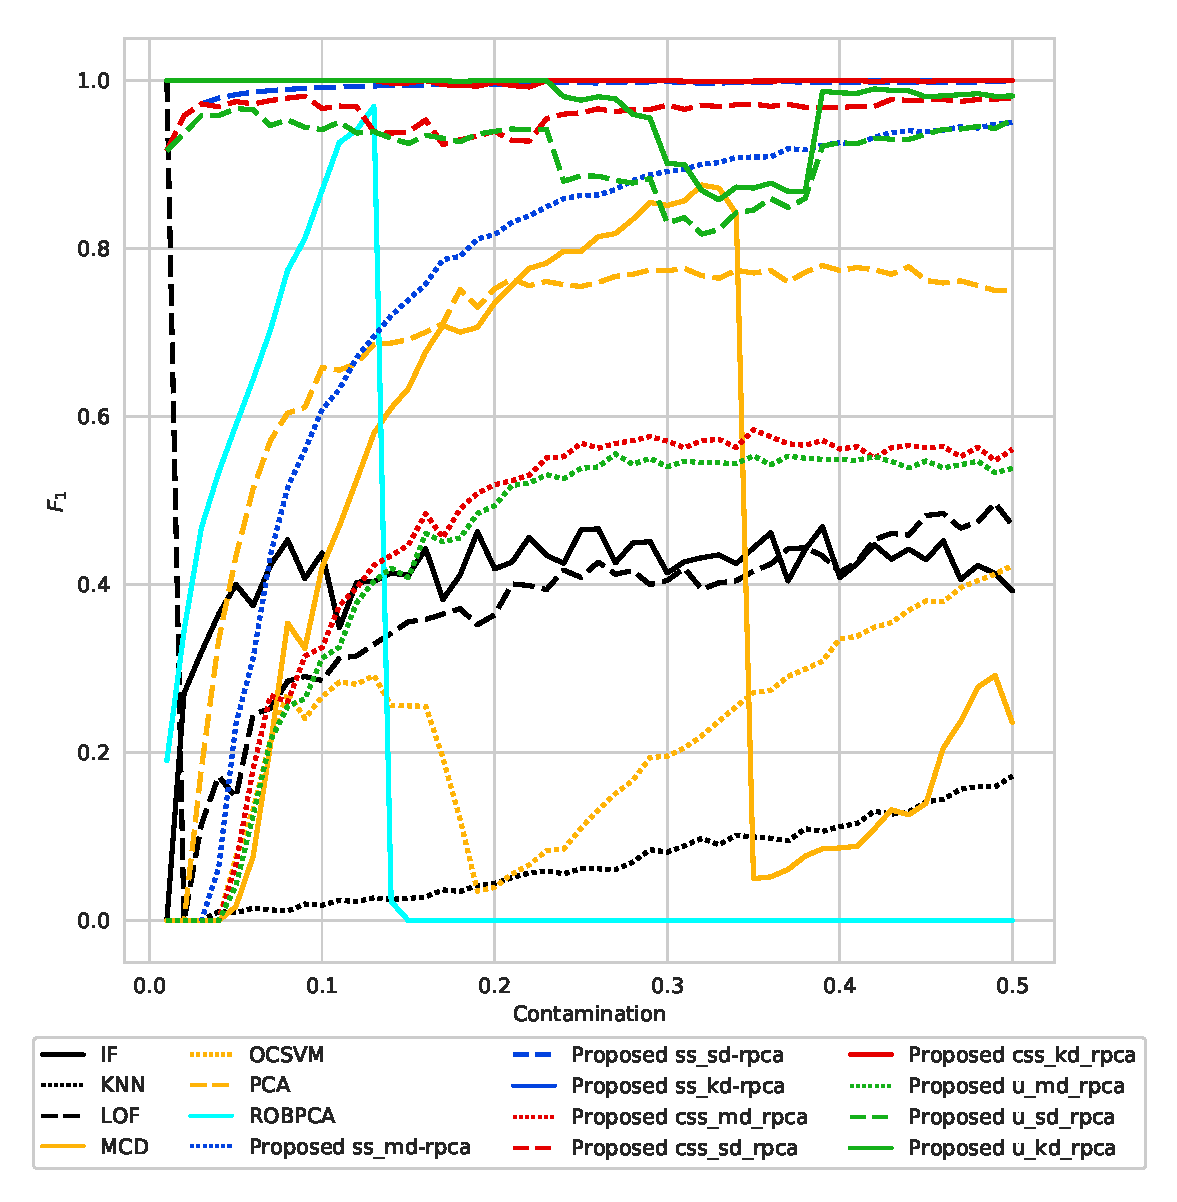
\includegraphics[width=8cm]{figures/ch4/pareto_f1_contamination.eps}
    	\caption{Anomaly detection on Pareto distributed with Gaussian anomalies}
    	\label{fig:4.11}
    \end{figure}
\end{frame}

\begin{frame}[c]{Results - Pareto with Gaussian anomalies}
	\begin{itemize}
		\item \textbf{kd-RPCA and sd-RPCA} obtained more than \textbf{0.8} $F_1$;
		\item The \textbf{contaminated semi-supervised of sd-RPCA and kd-RPCA} presented results \textbf{similar} to the \textbf{semi-supervised and unsupervised} approaches;
		\item The \textbf{unsupervised sd-RPCA and kd-RPCA} presented \textbf{better} results than widely adopted \textbf{unsupervised algorithms for outlier detection};
		\item The \textbf{semi-supervised kd-RPCA and sd-RPCA} obtained the \textbf{best} results.
	\end{itemize}
\end{frame}

\begin{frame}[c]{Results - Lognormal with Gaussian anomalies}
    \begin{figure}[h!]
    	\centering
    	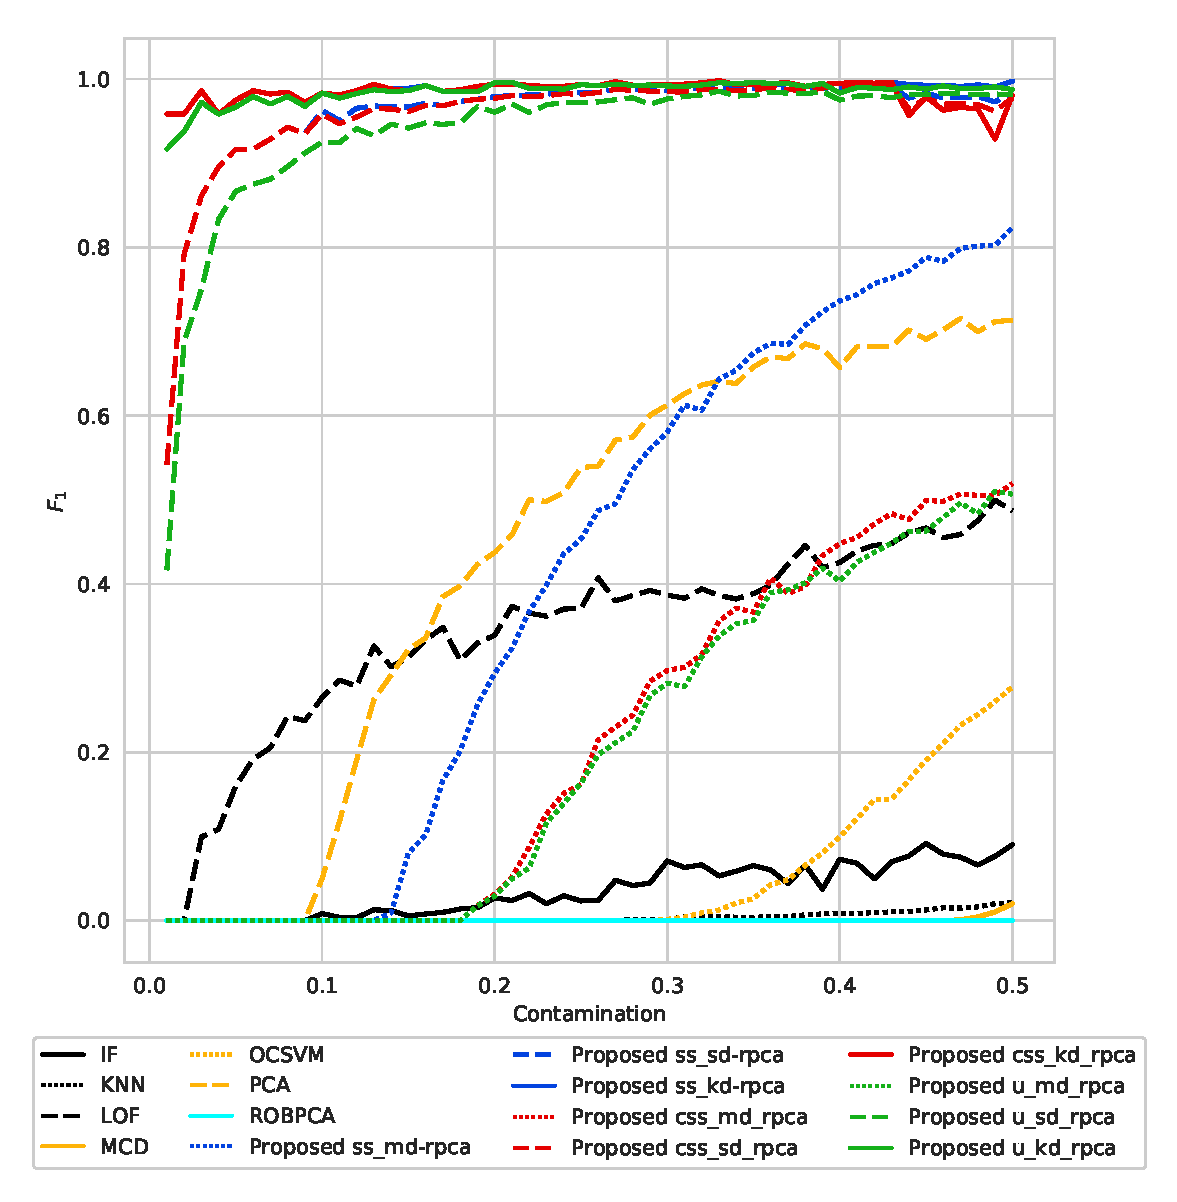
\includegraphics[width=8cm]{figures/ch4/lognormal_f1_contamination.eps}
    	\caption{Anomaly detection on Lognormal distributed with Gaussian anomalies}
    	\label{fig:4.12}
    \end{figure}
\end{frame}

\begin{frame}[c]{Results - Lognormal with Gaussian anomalies}
	\begin{itemize}
		\item \textbf{mean-based} approaches of \textbf{m-RPCA} presented \textbf{low} $F_1$;
		\item IF, KNN, LOF, MCD, OCSVM, PCA and ROBPCA were \textbf{worse than sd-RPCA and kd-RPCA};
		\item kd-RPCA performed better than sd-RPCA, with $F_1$ higher than 0.9.
	\end{itemize}
\end{frame}

\begin{frame}[c]{Results - Simulated data set}
    Conclusion:
    \begin{itemize}
        \item We can observe that mean-based approaches of m-RPCA are competitive for gaussian distributed data;
        \item The \textbf{robust subspace learning} of by md-RPCA, sd-RPCA and kd-RPCA, presented \textbf{higher anomaly detection} from \textbf{imbalanced and skewed} data than \textbf{widely adopted algorithms}. 
        \item The results refute the null hypothesis $H_2^{(N)}$ (\textbf{"An approach based on robust subspace learning does not improves the anomaly detection from imbalanced and skewed data"}).
	\end{itemize}
\end{frame}

\begin{frame}[c]{Experiments - CTU-13 data set}
    \textbf{Semi-supervised} approach of md-RPCA, sd-RPCA and kd-RPCA.
    
    Uniform \textbf{contamination} rate of \textbf{33\%}.
    
    m-RPCA is compared to:
    \begin{itemize}
        \item Isolation Forest (IF) \cite{liu2008isolation};
        \item k-Nearest Neighbors (KNN) \cite{angiulli2002fast};
        \item Local Outlier Factor (LOF) \cite{breunig2000lof};
        \item Minimum Covariance Deteminant (MCD) \cite{rousseeuw1999fastmcd};
        \item One-Class Support Vector Machines (OCSVM) \cite{scholkopf2001estimating};
        \item PCA \cite{shyu2003novel};
        \item ROBPCA-AO \cite{hubert2009robustskewed}.
	\end{itemize}
\end{frame}

\begin{frame}[c]{Results - CTU-13 data set}
    \begin{table}[h!]
      \centering
      \tiny
    %   \caption{Network anomaly detection from CTU-13 with 33\% of contamination}
      \label{tab:4.05}
      \begin{tabular}{ c|c|c|c|c|c|c|c }
    	\toprule
            \textbf{Algorithm}	&\textbf{10}	&\textbf{11}	&\textbf{12}	&\textbf{15}	&\textbf{15-2}	&\textbf{15-3}	&\textbf{16}	\\ \hline
            IF	&0.36	&0.34	&0.09	&0.21	&0.40	&0.44	&0.16\\ \hline
            KNN	&0.05	&0.17	&0.01	&0.03	&0.33	&0.23	&0.01\\ \hline
            LOF	&0.15	&0.14	&0.13	&0.17	&0.29	&0.22	&0.29\\ \hline
            MCD	&0.18	&0.29	&0.09	&0.34	&\color{red}\textbf{0.79}	&0.62	&0.04\\ \hline
            PCA	&0.33	&0.64	&0.69	&0.65	&0.55	&0.62	&0.75\\ \hline
            \color{red}\textbf{md-RPCA} &\color{red}\textbf{0.83}	&\color{red}\textbf{0.79}	&\color{red}\textbf{0.95}	&\color{blue}0.78	&\color{blue}0.78	&\color{red}\textbf{0.87}	&\color{red}\textbf{0.95}\\ \hline
            sd-RPCA &0.25	&0.75	&0.34	&0.64	&0.50	&0.75	&0.86\\ \hline
            kd-RPCA &0.76	&0.76	&0.90	&\color{red}\textbf{0.82}	&0.57	&0.76	&0.91\\ \hline
            ROBPCA-AO &0.01	&0.07	&0.00	&0.05	&0.38	&0.11	&0.05\\ \hline
        \bottomrule
      \end{tabular}
    \end{table}
    
        \begin{table}[h!]
      \centering
      \tiny
    %   \caption{Network anomaly detection from CTU-13 with 33\% of contamination}
      \label{tab:4.05}
      \begin{tabular}{ c|c|c|c|c|c|c|c }
    	\toprule
            \textbf{Algorithm}	&\textbf{16-2}	&\textbf{16-3}	&\textbf{17}	&\textbf{18}	&\textbf{18-2}	&\textbf{19}	&\textbf{Avg} \\ \hline
            IF	&0.34	&0.34	&0.41	&0.12	&0.16	&0.46	&0.29\\ \hline
            KNN	&0.25	&0.03	&0.12	&0.00	&0.00	&0.24	&0.11\\ \hline
            LOF	&0.38	&0.25	&0.24	&0.00	&0.04	&0.38	&0.21\\ \hline
            MCD	&0.58	&0.20	&0.41	&0.20	&0.20	&0.36	&0.33\\ \hline
            PCA	&0.50	&0.77	&0.33	&0.82	&0.01	&\color{red}\textbf{0.61}	&0.56\\ \hline
            \color{red}\textbf{md-RPCA} &\color{red}\textbf{0.87}	&\color{red}\textbf{0.80}	&\color{red}\textbf{0.82}	&\color{red}\textbf{0.83}	&\color{red}\textbf{0.82}	&\color{blue}0.51	&\color{red}\textbf{0.81}\\ \hline
            sd-RPCA &0.50	&0.77	&0.33	&0.82	&0.81	&0.21	&0.57\\ \hline
            kd-RPCA &0.50	&0.80	&0.73	&0.83	&0.81	&0.48	&0.74\\ \hline
            ROBPCA-AO &0.32	&0.03	&0.09	&0.07	&0.09	&0.21	&0.11\\ \hline
        \bottomrule
      \end{tabular}
    \end{table}
\end{frame}

\begin{frame}[c]{Results - CTU-13 data set}
	\begin{itemize}
		\item \textbf{md-RPCA, kd-RPCA and sd-RPCA overcome} the remain algorithms in \textbf{average} results;
		\item \textbf{md-RPCA} obtained the \textbf{best average} and the \textbf{best $F_1$ in 10 scenarios};
		\item The anomalies of the \textbf{scenario 19} are peer-to-peer botnet traffic generated by nsys.ay, which are related to botnet synchronization and \textbf{not to network attacks}.
	\end{itemize}
\end{frame}

%offline-=-=-=-=-=-=-=-=-=-=-=-=-=-=-=-=-=-=-=-=-=-=-=-=-=-=-=-=-=-=-=-=-=-=-=-=-=-=-=-=-=-=-=-=-=-=-=-=-=-=-=-
\section{Eigensimilarity for Anomaly Detection in Offline Mobile Client}
\label{Blocks}

\begin{frame}[c]{Introduction}
	\begin{itemize}
		\item According to \cite{khan2013towards, khan2015cloud}, the \textbf{state-of-the-art mobile cloud security models do not consider} the problem of the \textbf{offline security mode};
		\item Providers of the mobile security \textbf{avoid} the problem by completely \textbf{forbidding} the offline access.
	\end{itemize}
\end{frame}

\begin{frame}[c]{Introduction}
	In this work we present:
	\begin{itemize}
	    \item An \textbf{architecture and proof of concept of Eigensimilarity} for malicious behavior detection on mobile app;
		\item The common \textbf{threat} scenarios for \textbf{file cloud apps};
		\item The \textbf{performance} for \textbf{mobile} offline processing.
	\end{itemize}
\end{frame}

% \begin{frame}[c]{The mobile security architecture}
% 	\begin{figure}[h!]
% 		\centering
% 		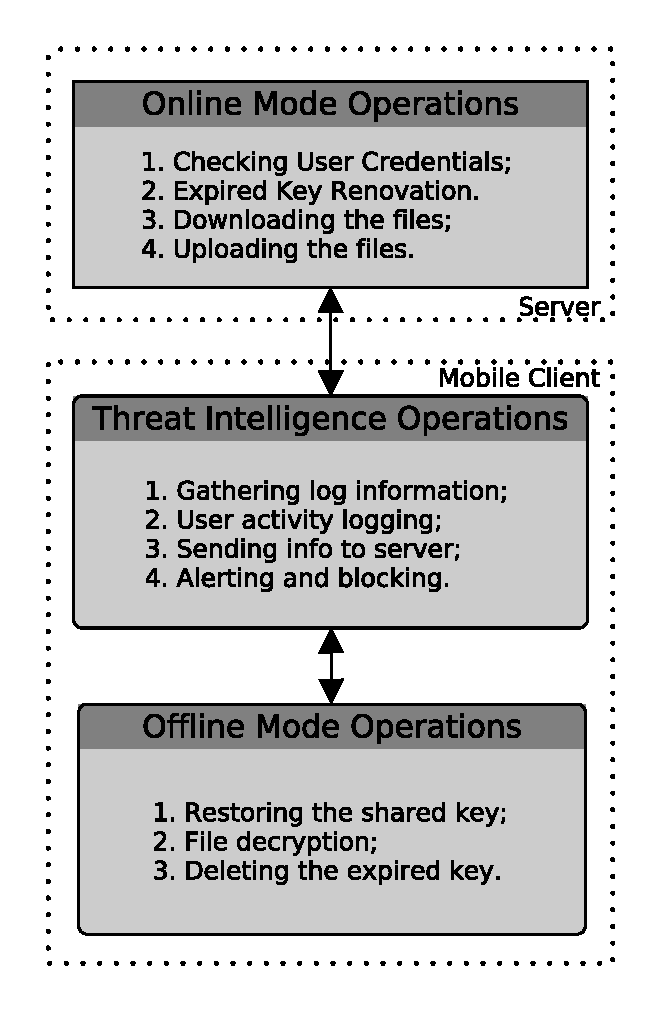
\includegraphics[width=5cm]{figures/ch3/fig01.eps}
% 		\caption{The core set of functions and protocols of the mobile cloud security infrastructure}
% 		\label{fig:3_01}
% 	\end{figure}
% \end{frame}

\begin{frame}[c]{Proposal for offline mobile security}
	\begin{figure}[h!]
		\centering
		\includegraphics[width=11cm]{figures/ch3/fig03.eps}
		\caption{Proposed Architecture for Offline Mobile Security}
		\label{fig:3_03}
	\end{figure}
\end{frame}

\begin{frame}[c]{Offline Behavioral Analysis}
	\begin{figure}[h!]
		\centering
		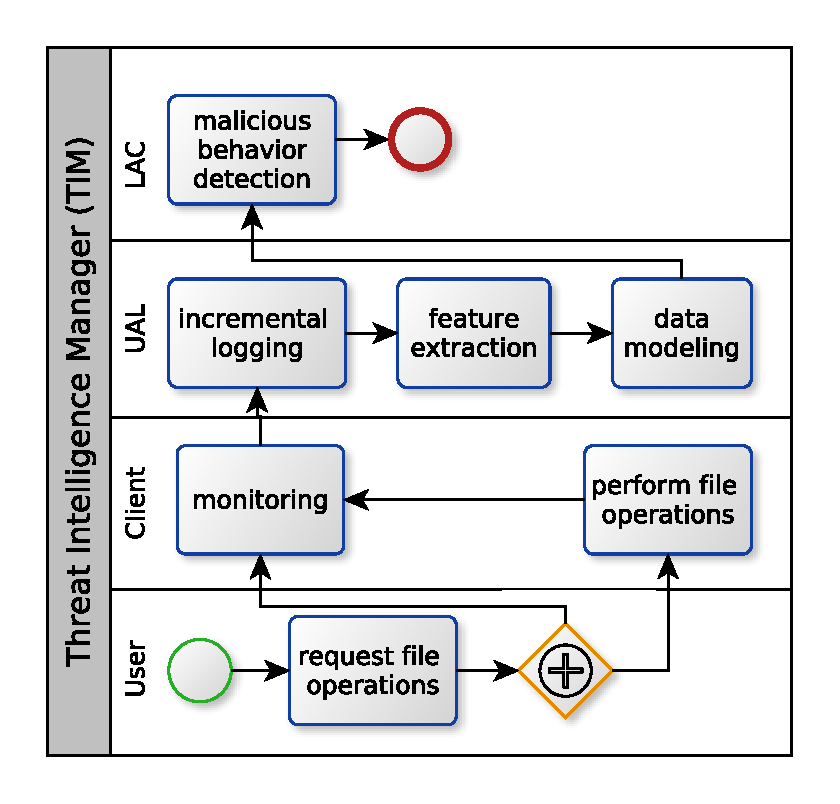
\includegraphics[width=7cm]{figures/ch3/fig06.eps}
		\caption{The Threat Intelligence Manager Workflow}
		\label{fig:3_06}
	\end{figure}
\end{frame}

\begin{frame}[c]{MOS for Threat Intelligence}
	\begin{itemize}
		\item Largest eigenvalue analysis and MOS (Previously presented);
		\item Applied to user behavior analysis;
		\begin{itemize}
			\item We model file operations as signals (matrices);
			\item We select features that can highlight malicious behaviors;
			\item We implement and evaluate into mobile devices.
		\end{itemize}
	\end{itemize}
\end{frame}

\begin{frame}[c]{Common threat scenarios}
	\begin{enumerate}
		\item An attacker uses a \textbf{valid password} to perform operations on a \textbf{bulk} of files.;
		\item Usage of \textbf{expired password} to perform unauthorized \textbf{operations};
	\end{enumerate}
\end{frame}

\begin{frame}[c]{Data Modeling for Behavioral Analysis}
	Selected features:
	\begin{itemize}
		\item File Access (Time and file system location);
		\item File Update (Time and file system location);
		\item File Download (Start time, end time and file system location);
		\item File Upload (Start time, end time and file system location).
	\end{itemize}
\end{frame}

% \begin{frame}[c]{Result: Data Modeling and Eigenvalue Analysis}
% 	\begin{table}
% 		\tiny
% 		\label{tab:3_04}
% 		\centering
% 		\begin{tabular}{|l|l|l|l|l|l|l|l|}
% 			\hline \rowcolor{Gray} Device	& \begin{tabular}[x]{@{}l@{}}Log Size\\(MB)\end{tabular}	& \begin{tabular}[x]{@{}l@{}}Window\\(min)\end{tabular}	& \begin{tabular}[x]{@{}l@{}}Modeling\\(ms)\end{tabular}	& \begin{tabular}[x]{@{}l@{}}Avg. Eig.\\(ms)\end{tabular}	& \begin{tabular}[x]{@{}l@{}}Std. Eig.\\(ms)\end{tabular}	& \begin{tabular}[x]{@{}l@{}}Eig. Min.\\(ms)\end{tabular}	& \begin{tabular}[x]{@{}l@{}}Eig. Max.\\(ms)\end{tabular}	\\ \hline
% 			Galaxy GT-I9300	& 6	& 60	& 107	& 209.52	& 18.58	& 183	& 276	\\ \hline
% 			Galaxy GT-I9300	& 6	& 40	& 115	& 227.26	& 18.13	& 191	& 289	\\ \hline
% 			Galaxy GT-I9300	& 6	& 20	& 89	& 268.14	& 21.94	& 229	& 315	\\ \hline
% 			Galaxy GT-I9300	& 6	& 10	& 90	& 347.42	& 24.11	& 304	& 421	\\ \hline
% 			Galaxy GT-I9300	& 4.1	& 60	& 20	& 60.90	& 15.19	& 37	& 106	\\ \hline
% 			Galaxy GT-I9300	& 4.1	& 40	& 20	& 68.72	& 15.71	& 43	& 114	\\ \hline
% 			Galaxy GT-I9300	& 4.1	& 20	& 34	& 89.04	& 16.78	& 54	& 133	\\ \hline
% 			Galaxy GT-I9300	& 4.1	& 10	& 21	& 117.24	& 14.36	& 96	& 171	\\ \hline
% 			Galaxy GT-I9300	& 1.4	& 60	& 10	& 159.82	& 15.82	& 125	& 197	\\ \hline
% 			Galaxy GT-I9300	& 1.4	& 40	& 10	& 168.06	& 15.90	& 139	& 220	\\ \hline
% 			Galaxy GT-I9300	& 1.4	& 20	& 11	& 204.4	& 20.46	& 176	& 269	\\ \hline
% 			Galaxy GT-I9300	& 1.4	& 10	& 13	& 259.00	& 21.34	& 220	& 315	\\ \hline
% 			Galaxy Tab SM-T800	& 6	& 60	& 7	& 59.30	& 6.55	& 54	& 74	\\ \hline
% 			Galaxy Tab SM-T800	& 6	& 40	& 8	& 62.56	& 7.05	& 56	& 80	\\ \hline
% 			Galaxy Tab SM-T800	& 6	& 20	& 10	& 73.28	& 8.59	& 65	& 95	\\ \hline
% 			Galaxy Tab SM-T800	& 6	& 10	& 8	& 93.48	& 9.13	& 83	& 130	\\ \hline
% 			Galaxy Tab SM-T800	& 4.1	& 60	& 11	& 18.64	& 4.51	& 16	& 38	\\ \hline
% 			Galaxy Tab SM-T800	& 4.1	& 40	& 11	& 19.64	& 5.12	& 17	& 38	\\ \hline
% 			Galaxy Tab SM-T800	& 4.1	& 20	& 12	& 25.12	& 5.55	& 21	& 46	\\ \hline
% 			Galaxy Tab SM-T800	& 4.1	& 10	& 12	& 32.32	& 7.29	& 27	& 55	\\ \hline
% 			Galaxy Tab SM-T800	& 1.4	& 60	& 4	& 49.08	& 6.01	& 42	& 62	\\ \hline
% 			Galaxy Tab SM-T800	& 1.4	& 40	& 5	& 51.42	& 7.36	& 44	& 74	\\ \hline
% 			Galaxy Tab SM-T800	& 1.4	& 20	& 5	& 51.12	& 7.80	& 54	& 91	\\ \hline
% 			Galaxy Tab SM-T800	& 1.4	& 10	& 7	& 75.24	& 7.71	& 65	& 90	\\ \hline
% 		\end{tabular}
% 	\end{table}
% \end{frame}

% \begin{frame}[c]{Result: EDC MOS}
% 	\begin{table}[!t]
% 		\tiny
% 		\label{tab:3_05}
% 		\centering
% 		\begin{tabular}{|l|l|l|l|l|l|l|l|}
% 			\hline \rowcolor{Gray} Device	& \begin{tabular}[x]{@{}l@{}}Log Size\\(MB)\end{tabular}	& \begin{tabular}[x]{@{}l@{}}Window\\(min)\end{tabular}	& \begin{tabular}[x]{@{}l@{}}Avg. EDC.\\(ms)\end{tabular}	& \begin{tabular}[x]{@{}l@{}}Std. EDC.\\(ms)\end{tabular}	& \begin{tabular}[x]{@{}l@{}}Min. EDC.\\(ms)\end{tabular}	& \begin{tabular}[x]{@{}l@{}}Max. EDC.\\(ms)\end{tabular}	\\ \hline
% 			Galaxy GT-I9300	& 6	& 60	& 5.27	& 4.04	& 3	& 20	\\ \hline
% 			Galaxy GT-I9300	& 6	& 40	& 10.78	& 6.37	& 6	& 34	\\ \hline
% 			Galaxy GT-I9300	& 6	& 20	& 32.62	& 12.44	& 21	& 88	\\ \hline
% 			Galaxy GT-I9300	& 6	& 10	& 115.08	& 17.45	& 88	& 158	\\ \hline
% 			Galaxy GT-I9300	& 4.1	& 60	& 5.68	& 4.18	& 3	& 23	\\ \hline
% 			Galaxy GT-I9300	& 4.1	& 40	& 10.76	& 5.31	& 7	& 27	\\ \hline
% 			Galaxy GT-I9300	& 4.1	& 20	& 37.58	& 10.30	& 23	& 61	\\ \hline
% 			Galaxy GT-I9300	& 4.1	& 10	& 125.98	& 18.56	& 101	& 191	\\ \hline
% 			Galaxy GT-I9300	& 1.4	& 60	& 4.92	& 3.49	& 3	& 17	\\ \hline
% 			Galaxy GT-I9300	& 1.4	& 40	& 9.00	& 4.23	& 6	& 25	\\ \hline
% 			Galaxy GT-I9300	& 1.4	& 20	& 30.14	& 9.21	& 19	& 62	\\ \hline
% 			Galaxy GT-I9300	& 1.4	& 10	& 100.62	& 15.83	& 69	& 163	\\ \hline
% 			Galaxy Tab SM-T800	& 6	& 60	& 1.84	& 0.65	& 1	& 3	\\ \hline
% 			Galaxy Tab SM-T800	& 6	& 40	& 3.26	& 1.24	& 2	& 7	\\ \hline
% 			Galaxy Tab SM-T800	& 6	& 20	& 10.90	& 2.40	& 9	& 21	\\ \hline
% 			Galaxy Tab SM-T800	& 6	& 10	& 41.86	& 7.33	& 34	& 60	\\ \hline
% 			Galaxy Tab SM-T800	& 4.1	& 60	& 1.85	& 0.60	& 1	& 3	\\ \hline
% 			Galaxy Tab SM-T800	& 4.1	& 40	& 3.62	& 1.10	& 2	& 8	\\ \hline
% 			Galaxy Tab SM-T800	& 4.1	& 20	& 12.04	& 2.79	& 9	& 22	\\ \hline
% 			Galaxy Tab SM-T800	& 4.1	& 10	& 40.16	& 6.48	& 35	& 60	\\ \hline
% 			Galaxy Tab SM-T800	& 1.4	& 60	& 1.98	& 0.89	& 1	& 6	\\ \hline
% 			Galaxy Tab SM-T800	& 1.4	& 40	& 3.30	& 1.16	& 2	& 7	\\ \hline
% 			Galaxy Tab SM-T800	& 1.4	& 20	& 10.48	& 2.90	& 8	& 21	\\ \hline
% 			Galaxy Tab SM-T800	& 1.4	& 10	& 34.52	& 4.08	& 30	& 45	\\ \hline
% 		\end{tabular}
% 	\end{table}
% \end{frame}

\begin{frame}[c]{Results - synthetic data set}
	\begin{itemize}
		\item The \textbf{highest eigenvalue analysis} time: \textbf{421ms} with average of \textbf{347.42ms};
		\item The \textbf{lower window} size leads to the \textbf{larger eigenvalue analysis time};
		\item The \textbf{MOS} processing time \textbf{increases} with the \textbf{window size decreasing};
		\item The \textbf{highest MOS} processing time: lower than \textbf{200s};
		\item This results represent an \textbf{acceptable processing time} for \textbf{anomaly detection in mobile clients}.
	\end{itemize}
\end{frame}


%section-=-=-=-=-=-=-=-=-=-=-=-=-=-=-=-=-=-=-=-=-=-=-=-=-=-=-=-=-=-=-=-=-=-=-=-=-=-=-=-=-=-=-=-=-=-=-=-=-=-=-=-
\section{Conclusion}

\begin{frame}[c]{Conclusion}
	\begin{itemize}
		\item \textbf{Synflood, fraggle and port scan} attacks can be \textbf{detected} accurately and with great detail by \textbf{Eigensimilarity}, in an automatic and \textbf{blind} fashion;
		\item As \textbf{proof of concept}, a mobile app was developed to test the \textbf{security solution}, with positive \textbf{results} in terms of \textbf{performance};
	\end{itemize}
\end{frame}

\begin{frame}[c]{Conclusion}
	\begin{itemize}
		\item \textbf{m-RPCA} can \textbf{improve the anomaly detection on skewed and imbalanced data set}. 
		\item \textbf{m-RPCA} can be adopted for \textbf{network attack detection}, with \textbf{better} results than \textbf{widely adopted algorithms for outlier detection}; 
	\end{itemize}
\end{frame}

%section-=-=-=-=-=-=-=-=-=-=-=-=-=-=-=-=-=-=-=-=-=-=-=-=-=-=-=-=-=-=-=-=-=-=-=-=-=-=-=-=-=-=-=-=-=-=-=-=-=-=-=-
\begin{frame}[plain, allowframebreaks]{Bibliography}
	\setbeamertemplate{bibliography item}[text]
	\printbibliography
\end{frame}

\end{document}
